%%%%%%%%%%%%%%%%%%%%%%%%%%%%%%%%%%%%%%%%%
% Masters/Doctoral Thesis 
% LaTeX Template
% Version 2.5 (27/8/17)
%
% This template was downloaded from:
% http://www.LaTeXTemplates.com
%
% Version 2.x major modifications by:
% Vel (vel@latextemplates.com)
%
% This template is based on a template by:
% Steve Gunn (http://users.ecs.soton.ac.uk/srg/softwaretools/document/templates/)
% Sunil Patel (http://www.sunilpatel.co.uk/thesis-template/)
%
% Template license:
% CC BY-NC-SA 3.0 (http://creativecommons.org/licenses/by-nc-sa/3.0/)
%
%%%%%%%%%%%%%%%%%%%%%%%%%%%%%%%%%%%%%%%%%


%----------------------------------------------------------------------------------------
%	PACKAGES AND OTHER DOCUMENT CONFIGURATIONS
%----------------------------------------------------------------------------------------

\documentclass[
11pt, % The default document font size, options: 10pt, 11pt, 12pt
%oneside, % Two side (alternating margins) for binding by default, uncomment to switch to one side
% serbian, % ngerman for German
serbian,
singlespacing, % Single line spacing, alternatives: onehalfspacing or doublespacing
%draft, % Uncomment to enable draft mode (no pictures, no links, overfull hboxes indicated)
%nolistspacing, % If the document is onehalfspacing or doublespacing, uncomment this to set spacing in lists to single
%liststotoc, % Uncomment to add the list of figures/tables/etc to the table of contents
%toctotoc, % Uncomment to add the main table of contents to the table of contents
%parskip, % Uncomment to add space between paragraphs
% nohyperref, % Uncomment to not load the hyperref package
headsepline, % Uncomment to get a line under the header
%chapterinoneline, % Uncomment to place the chapter title next to the number on one line
%consistentlayout, % Uncomment to change the layout of the declaration, abstract and acknowledgements pages to match the default layout
]{MastersDoctoralThesis} % The class file specifying the document structure

 
\usepackage[utf8]{inputenc} % Required for inputting international characters
\usepackage[T1]{fontenc} % Output font encoding for international characters

\usepackage{mathpazo} % Use the Palatino font by default
\usepackage{amsmath}
% dužine

\usepackage{listings}                                                           
\usepackage{color}

\definecolor{mygreen}{rgb}{0,0.6,0}
\definecolor{mygray}{rgb}{0.5,0.5,0.5}
\definecolor{mymauve}{rgb}{0.58,0,0.82}

                                                                                

% \usepackage[backend=bibtex,style=authoryear,natbib=true]{biblatex} % Use the bibtex backend with the authoryear citation style (which resembles APA)
\usepackage[
  backend=bibtex
  , natbib=true
  , citestyle=numeric
  , bibstyle=numeric
  , sorting=none
  , maxbibnames=99
]{biblatex} % Use the bibtex backend with the authoryear citation style (which resembles APA)


\addbibresource{ref.bib} % The filename of the bibliography


% \usepackage[autostyle=true]{csquotes} % Required to generate language-dependent quotes in the bibliography

%----------------------------------------------------------------------------------------
%	MARGIN SETTINGS
%----------------------------------------------------------------------------------------

\geometry{
	paper=a4paper, % Change to letterpaper for US letter
	% inner=3.15cm, % Inner margin
	% outer=3.15cm, % Outer margin
	% bindingoffset=0cm, % Binding offset
	inner=2.5cm, % Inner margin
	outer=3.8cm, % Outer margin
	bindingoffset=.5cm, % Binding offset
	top=1.5cm, % Top margin
	bottom=1.5cm, % Bottom margin
  % showframe, % Uncomment to show how the type block is set on the page
}

%----------------------------------------------------------------------------------------
%	THESIS INFORMATION
%----------------------------------------------------------------------------------------

\thesistitle{Bioinformatička analiza povezanosti funkcije i neuređenosti proteina} % Your thesis title, this is used in the title and abstract, print it elsewhere with \ttitle

\supervisor{dr Jovana \textsc{Kovačević}} % Your supervisor's name, this is used in the title page, print it elsewhere with \supname
\examiner{} % Your examiner's name, this is not currently used anywhere in the template, print it elsewhere with \examname
\degree{Master informatičar} % Your degree name, this is used in the title page and abstract, print it elsewhere with \degreename
\author{Goran \textsc{Vinterhalter}} % Your name, this is used in the title page and abstract, print it elsewhere with \authorname
\addresses{https://www.linkedin.com/in/goran-vinterhalter-6996a412b/} % Your address, this is not currently used anywhere in the template, print it elsewhere with \addressname

\subject{Bioinformatika} % Your subject area, this is not currently used anywhere in the template, print it elsewhere with \subjectname
\keywords{} % Keywords for your thesis, this is not currently used anywhere in the template, print it elsewhere with \keywordnames
\university{\href{http://www.bg.ac.rs}{Univerzitet u Beogradu}} % Your university's name and URL, this is used in the title page and abstract, print it elsewhere with \univname
\department{\href{http://www.racunarstvo.matf.bg.ac.rs/}{Katedra za Računarstvo i informatiku}} % Your department's name and URL, this is used in the title page and abstract, print it elsewhere with \deptname
\group{.} % Your research group's name and URL, this is used in the title page, print it elsewhere with \groupname
% \group{\href{http://researchgroup.university.com}{Research Group Name}} % Your research group's name and URL, this is used in the title page, print it elsewhere with \groupname
\faculty{\href{http://matf.bg.ac.rs}{Matematički fakultet}} % Your faculty's name and URL, this is used in the title page and abstract, print it elsewhere with \facname

\AtBeginDocument{
\hypersetup{pdftitle=\ttitle} % Set the PDF's title to your title
\hypersetup{pdfauthor=\authorname} % Set the PDF's author to your name
\hypersetup{pdfkeywords=\keywordnames} % Set the PDF's keywords to your keywords
}

\begin{document}

\frontmatter % Use roman page numbering style (i, ii, iii, iv...) for the pre-content pages

\pagestyle{plain} % Default to the plain heading style until the thesis style is called for the body content

%----------------------------------------------------------------------------------------
%	TITLE PAGE
%----------------------------------------------------------------------------------------

\begin{titlepage}
\begin{center}

\vspace*{.06\textheight}
{\scshape\LARGE \univname\par} % University name
{\scshape\LARGE \facname\par} % University name
\vspace{1.5cm}
\textsc{\Large Master Rad}\\[0.5cm] % Thesis type

\HRule \\[0.4cm] % Horizontal line
{\huge \bfseries \ttitle\par}\vspace{0.4cm} % Thesis title
\HRule \\[1.5cm] % Horizontal line
 
\begin{minipage}[t]{0.4\textwidth}
\begin{flushleft} \large
\emph{Autor:}\\
\href{https://www.linkedin.com/in/goran-vinterhalter-6996a412b/}{\authorname} % Author name - remove the \href bracket to remove the link
\end{flushleft}
\end{minipage}
\begin{minipage}[t]{0.4\textwidth}
\begin{flushright} \large
\emph{Mentor:} \\
\href{http://poincare.matf.bg.ac.rs/~jovana/}{\supname} % Supervisor name - remove the \href bracket to remove the link  
\end{flushright}
\end{minipage}\\[2cm]
 
\vfill

% \large \textit{A thesis submitted in fulfillment of the requirements\\ for the degree of \degreename}\\[0.3cm] % University requirement text
% \textit{in the}\\[0.4cm]
% \groupname\\\deptname\\[2cm] % Research group name and department name

{\scshape\LARGE Članovi komsije:\par}\vspace{0.2cm} % University name
prof. dr Gordana Pavlović-Lažetić \\
prof. dr Saša Malkov \\
doc. dr Jovana Kovačević \\

 
\vfill

\vspace{1cm}
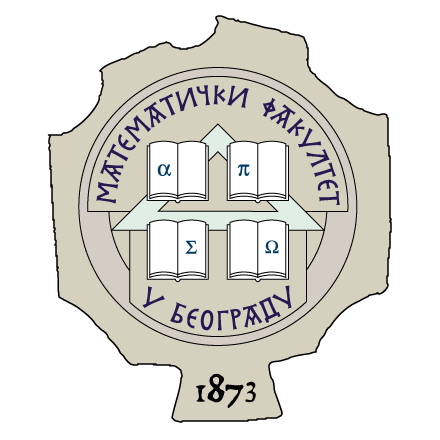
\includegraphics[scale=0.25]{Logo}\\ % University/department logo - uncomment to place it
\vspace{0.5cm}
{\large Beograd, 2018}\\ % Date
 
\vfill
\end{center}
\end{titlepage}

%----------------------------------------------------------------------------------------
%	DECLARATION PAGE
%----------------------------------------------------------------------------------------

% \begin{declaration}
% \addchaptertocentry{\authorshipname} % Add the declaration to the table of contents
% \noindent I, \authorname, declare that this thesis titled, \enquote{\ttitle} and the work presented in it are my own. I confirm that:
%
% \begin{itemize} 
% \item This work was done wholly or mainly while in candidature for a research degree at this University.
% \item Where any part of this thesis has previously been submitted for a degree or any other qualification at this University or any other institution, this has been clearly stated.
% \item Where I have consulted the published work of others, this is always clearly attributed.
% \item Where I have quoted from the work of others, the source is always given. With the exception of such quotations, this thesis is entirely my own work.
% \item I have acknowledged all main sources of help.
% \item Where the thesis is based on work done by myself jointly with others, I have made clear exactly what was done by others and what I have contributed myself.\\
% \end{itemize}
%  
% \noindent Signed:\\
% \rule[0.5em]{25em}{0.5pt} % This prints a line for the signature
%  
% \noindent Date:\\
% \rule[0.5em]{25em}{0.5pt} % This prints a line to write the date
% \end{declaration}
%
% \cleardoublepage

%----------------------------------------------------------------------------------------
%	QUOTATION PAGE
%----------------------------------------------------------------------------------------

% \vspace*{0.2\textheight}
%
% \noindent\enquote{\itshape Thanks to my solid academic training, today I can write hundreds of words on virtually any topic without possessing a shred of information, which is how I got a good job in journalism.}\bigbreak
%
% \hfill Dave Barry

%----------------------------------------------------------------------------------------
%	ABSTRACT PAGE
%----------------------------------------------------------------------------------------

% definišemo korisne komande
\newcommand{\en}[1]{(engl. \textit{#1})}
\newcommand{\lat}[1]{(latin. \textit{#1})}
\newcommand{\keyword}[1]{\textbf{#1}}
\newcommand{\ikeyword}[1]{\textit{\textbf{#1}}}
\newcommand{\tabhead}[1]{\textbf{#1}}
\newcommand{\code}[1]{\texttt{#1}}
\newcommand{\file}[1]{\texttt{\bfseries#1}}
\newcommand{\option}[1]{\texttt{\itshape#1}}


\newcommand{\uniprot}{\textit{UniProt} }
\newcommand{\uniprotkb}{\textit{UniProtKB} }
\newcommand{\swissprot}{\textit{Swiss-Prot} }
\newcommand{\trembl}{\textit{TrEMBL} }

\newcommand{\kw}[1]{\textbf{\textit{KW: #1}}}
\newcommand{\mf}[1]{\textbf{\textit{MF: #1}}}

\newtheorem{definicija}{Definicija}

\begin{abstract}
\addchaptertocentry{\abstractname} % Add the abstract to the table of contents
% The Thesis Abstract is written here (and usually kept to just this page). The page is kept centered vertically so can expand into the blank space above the title too\ldots



Korelacija između molekulske funkcije proteina i inherentne neuređenosti
predstavlja bitan aspekt izučavanja odnosa (zavisnosti) između funkcije,
sekvence i strukture.
Istraživanje u ovom radu je inspirisano statističkom metodom za ocenu
korelacije predloženom u referentnom radu \textit{Xie et al.} \cite{Xie2007}.
U navedenom radu izučen je odnos između strukture i funkcije  proteina pri čemu
su proteini preuzeti iz baze \swissprot a funkcije opisane ključnim
Svis-Prot-rečima (ključnim rečima).

U ovom radu skup proteina čini trening skup sa CAFA3 takmičenja, dok su
funkcije pored ključnih reči opisane i terminima molekulske funkcije iz
ontologije gena (GO-termini).  Analiza je izvedena i nad ključnim rečima i nad
GO-terminima, ali je ograničena (respektivno) na kategoriju molekulskih
funkcija (MF). 

Prediktor PONDR VSL2b korišćen je za karakterizaciju preko 66000 CAFA3-proteina
kao putativno uređenih ili neuređenih, dok su funkcijske anotacije (ključne
reči i GO-termini) preuzete iz \swissprot baze.  Od 186 ključnih MF-reči  koje
anotiraju minimum 20 proteina, utvrđeno je da su 53 korelirane sa uređenim, a
44 sa neuređenim proteinima. Pod istim uslovima, od 1781 MF-termin 699 je
korelirano sa uređenim, a 616 sa neuređenim proteinima. Dodatno, rezultati
MF-termina predstavljeni su kao interaktivni graf koji prikazuje kompleksnu
hijerarhijsku strukturu ontologije gena.
Dobijeni rezultati nad ključnim MF-rečima  upoređeni su sa rezultatima iz
referentnog rada i upoređeni su sa rezultatima nad MF-terminima.  Komparacija
dve funkcijske nomenklature, GO i ključne reči, pokazala je konzistentne
rezultate za adekvatna preslikavanja. Međutim, komparacija referentnih i novih
rezultata otkrila je da funkcije koje opisuju molekulsko vezivanje preovlađuju
među novim rezultatima (neuređenih funkcija) dok se u starim rezultatima ne
javljaju.  Zbog malog broja poznatih veza u preslikavanju između ključnih reči
i GO-termina, predložena je nova metoda za izvođenje najverovatnijih
nedostajućih veza tako što se verovatnoća ocenjuje sličnošću (Žakardov indeks)
između skupova proteina anotiranih različitim funkcijama.  Pored toga, metod iz
referentog rada dopunjen je saznanjem da se pod istim uslovima korelacija
između dužine proteina i njegove klasifikacije (kao putativno neuređenog) može
aproksimirati i slučajno generisanim proteinskim sekvencama.




\end{abstract}




%----------------------------------------------------------------------------------------
%	ACKNOWLEDGEMENTS
%----------------------------------------------------------------------------------------

% \begin{acknowledgements}
% \addchaptertocentry{\acknowledgementname} % Add the acknowledgements to the table of contents
% The acknowledgments and the people to thank go here, don't forget to include your project advisor\ldots
% \end{acknowledgements}
%
%----------------------------------------------------------------------------------------
%	LIST OF CONTENTS/FIGURES/TABLES PAGES
%----------------------------------------------------------------------------------------

\tableofcontents % Prints the main table of contents

% \listoffigures % Prints the list of figures

% \listoftables % Prints the list of tables

%----------------------------------------------------------------------------------------
%	ABBREVIATIONS
%----------------------------------------------------------------------------------------

% \begin{abbreviations}{ll} % Include a list of abbreviations (a table of two columns)
%
% \textbf{LAH} & \textbf{L}ist \textbf{A}bbreviations \textbf{H}ere\\
% \textbf{WSF} & \textbf{W}hat (it) \textbf{S}tands \textbf{F}or\\
%
% \end{abbreviations}

%----------------------------------------------------------------------------------------
%	PHYSICAL CONSTANTS/OTHER DEFINITIONS
%----------------------------------------------------------------------------------------

% \begin{constants}{lr@{${}={}$}l} % The list of physical constants is a three column table
%
% % The \SI{}{} command is provided by the siunitx package, see its documentation for instructions on how to use it
%
% Speed of Light & $c_{0}$ & \SI{2.99792458e8}{\meter\per\second} (exact)\\
% %Constant Name & $Symbol$ & $Constant Value$ with units\\
%
% \end{constants}

%----------------------------------------------------------------------------------------
%	SYMBOLS
%----------------------------------------------------------------------------------------

% \begin{symbols}{lll} % Include a list of Symbols (a three column table)
%
% $a$ & distance & \si{\meter} \\
% $P$ & power & \si{\watt} (\si{\joule\per\second}) \\
% %Symbol & Name & Unit \\
%
% \addlinespace % Gap to separate the Roman symbols from the Greek
%
% $\omega$ & angular frequency & \si{\radian} \\
%
% \end{symbols}

%----------------------------------------------------------------------------------------
%	DEDICATION
%----------------------------------------------------------------------------------------

% \dedicatory{For/Dedicated to/To my\ldots} 

%----------------------------------------------------------------------------------------
%	THESIS CONTENT - CHAPTERS
%----------------------------------------------------------------------------------------

\mainmatter % Begin numeric (1,2,3...) page numbering

\pagestyle{thesis} % Return the page headers back to the "thesis" style



% Include the chapters of the thesis as separate files from the Chapters folder
% Uncomment the lines as you write the chapters


\chapter{Uvod} % Main chapter title

\label{Uvod} % For referencing 


%------------------------------------------------------------------------------

\section{Osnovni biološki  pojmovi}

Svi živi organizmi sastoje se od jedne ili više ćelija, a svaka ćelija od
molekula. Veliki \footnote{ Obično se molekulska masa od $1000 Da$ (Daltona) uzima kao 
granica između malih molekula i makromolekula.}
molekuli (makromolekuli) organskog porekla obično \footnote{
  Lipidi recimo nisu polimeri, ali su principijalno slični
} su sačinjeni od
ponavljajućih strukturnih jedinica \keyword{monomera} \textit{(mono- = jedan,
mer- = deo)} međusobno povezanih \keyword{kovalentnim} vezama.  Takav molekul
zovemo \keyword{polimer} \textit{(poli- =mnogo, -mer= deo)}. 
% Polimer može da bude \textit{homo-polimer}, sačinjen od jednog tipa monomera
% ili suprotno \textit{hetero-polimer}, sačinjen od nekoliko raznih tipova
% monomera.
Skup monomera možemo da smatramo azbukom koja gradi jezik polimera.  Mali broj
monomera je dovoljan za strukturnu kompleksnost bilo koje ćelije.  Tri 
najznačajnija tipa bioloških polimera i njihovi monomeri prikazani su u Tabli
\ref{tab:polimeri}.

\begin{table}[htpb]
  \centering
  \caption{Najznačajniji biološki polimeri}
  \label{tab:polimeri}
  \begin{tabular}{ll}
    \keyword{Polimer}            & \keyword{Monomer} \\
    Ugljeni hidrati              & Monosaharid (šećeri) \\
    Nukleinska kiselina (DNK)    & Nukleotid \\
    Protein                      & Aminokiselina \\
    \hline
  \end{tabular}
\end{table}



\label{sec:}
\subsection{Proteini}

Proteini su najčešći biološki makromolekuli koji čine i do $80\%$ suve mase
organizma.  Strukturno protein je linearan polimeri sačinjen od lanca
\keyword{aminokiselina}(monomeri). 





\chapter{Inherentno neuređeni proteini} % Main chapter title

\label{IDP} % For referencing 


Funkcionalni proteini sa delimičnim ili potpunim izostankom strukture (pri
fiziološkim uslovima) nalaze se svuda u živom svetu, do te mere da ima više
smisla upitati ''gde se oni ne nalaze?'' nego obratno \parencite{uversky2016}.
Danas neuređenost proteina je uzrokovala nastanak velikog broj hipoteza, od
$D^2$ koncepta bolesti \parencite{Uversky2008} pa sve do evolucije
višećelijskih organizama \parencite{Romero2006} i osobina prvih oblika života
\parencite{Trifonov2000, uversky2016}. Šta više, sa početkom 21. veka broj
naučnih radova koji se bave ovom temom doživljava skoro eksponencijalan
porast \parencite{oldfield2014},ali  da bi se razumela popularnost i 
perspektiva koju polje donosi neophodno je osvrnuti se na istoriju.

Fišerova\footnote{ Emil Fišer bio je Nemački hemičar koji je 1894. predložio
analogiju brave i ključa opisujući karakteristike enzima pivske
plesni \parencite{dunker2001}.  } analogija o \keyword{bravi i ključu} ponovo
otkrivena nezavisnim istraživanjima Hsien Wu,  Mirski i Paulinga 
postavila je temelje ''opšteprihvaćene''
\keyword{struktura-funkcija} paradigme \parencite{dunker2001}.
% ''
% Specifične osobine nativnih\ref{} proteina mi pripisujemo njihovoj jedinstveno
% definisanoj konfiguraciji.  Denaturisane proteine mi smatramo okarakterisane
% izostankom jedinstveno definisane konfiguracije
% ''(Mirski i Pauling)
\textit{“The characteristic specific properties of native\footnote{ nativno stanje
  proteina je savijeno, operativno, funkcionalno stanje \parencite{dunker2001}.
Ovaj termin bio je isprepleten sa paradigmom struktura-funkcija} proteins we
attribute to their uniquely defined configurations. The denatured protein
molecule we consider to be characterized by the absence of a uniquely defined
configuration”} \parencite{MirskyPauling1936}. Predloženi model prilagođen je
funkcionisanju enzima, čija sposobnost da katalizuju zavisi od jasno
definisanog geometriskog oblika koji moraju da zauzmu odnosno u koji moraju da
se saviju.  Substrat (ključ ili funkcija) diktira oblik enzima (brave ili
strukture) \parencite{biology}.  Kontrapozicijom sledi da nedostatak strukture
vodi izostanku funkcije.

Prvi kontraprimer navedene teorije javio se još 1950. Protein krvne plazme, serum
albumin pokazivao je veliku mogućnost vezivanja za različite
partnere \parencite{dunker2001}. Ovo otkriće ukazivalo je da specifične zahteve
enzima ne treba generalizovati na sve proteine. Ipak model brave i ključ i
njena poboljšana varijanta \keyword{teorija indukovanog fita}\footnote{ Teorija
indukovanog fita omekšava rigidnost modela brava-ključ sugerišući da interakcija
sa substratom indukuje konačni oblik enzima maksimizujući
reakciju \parencite{biology}} \en{induced-fit theory} dominirale su krajem
prošlog veka, zanemarujuću konstantno rastući skup funkcionalnih
''ne-nativnih'' proteina čije postojanje nisu mogle da objasne. Sa druge strane
tehnološki napretci u razlučivanju strukture proteina jasno su demonstrirali
obimno postojanje funkcionalnih proteina bez uređene 3D strukture (pri
fiziološkim uslovima)  od kojih su neki bili neuređeni celom
dužinom \parencite{dunker2001}.  Nova paradigma je bila neophodan.

Hipoteza proteinskog trojstva \parencite{dunker2001} (nastala tek početkom
21. veka) predlaže da funkcija proteina može zavisiti od bilo kojeg od tri
stanja ili tranzicije između tih stanja. Predložena stanja predstavljaju
nativne oblike proteina i analogna su najčešćim stanjima materije na zemlji.
Model je naknadno dopunjen još jednim stanjem:
\begin{enumerate}
  \item \keyword{Uređen protein} - čvrsto stanje

  \item \keyword{Topljiva globula} \en{molten globule} - tečno stanje

  \item \keyword{Pre-topljiva globula} \en{pre-molten globule} - međustanje\\ 
    Usled nejasne tranzicije između stanja topljivog globula i nasumičnog
    klupka (suprotno analogiji tečnog i gasovitog stanja) \parencite{dunker2001}
    model je dopunjen.

  \item \keyword{Nasumično klupko} \en{random coil} - gasovito stanje
\end{enumerate}

Povezanost sekvence sa strukturom sugeriše da je neuređenost enkodirano
inherentno\footnote{ Inherentno ili prirođeno, nasleđeno} svojstvo \parencite{dunker2001}
stoga ove proteine nazivamo \keyword{Inherentno\footnote{ U nedostatku
    adekvatne domaće reči koristimo najbliži sinonim reči \en{intrinsic} tj.
\en{inherent}, koja čuva suštinu originalnog značenja.  } Neuređeni Proteini}
\en{Intrinsically Disorderd Proteins} skraćeno \keyword{IDP}, a njihove neuređene
ali funkcionalne regione \keyword{IDPr} \parencite{uversky2016}. U ovom radu pod
neuređenošću proteina podrazumevaćemo inherentnu neuređenost osim ako to nije
drugačije naglašeno\footnote{ tumačenje neuređenosti zavisi od konteksta i može
  da označava denaturisane ili na drugi način dobijene nefunkcionalne
proteine}.

Današnje procene zastupljenosti pronašle su da 19\% aminokiselina kod
eukariota, 6\% kod bakterija i 4\% kod arhea pripadaju
IDPr \parencite{Peng2014}.  Čak 50\% proteina eukariota ima bar jedan IDPr duži
ili jednak od 30 uzastopnih AK \parencite{Xue2012} dok je za 6\% do 17\%
predviđeno da su neurđeni celom dužinom \parencite{Tompa2002}.  Ovi podaci bude
veliko interesovanje naučnika da istraže funkciju i ponašanje IDP i IDPr.

\section {Osobine i uticaj na funkciju}

Detaljno opisivanje osobina i posledica neuređenosti prevazilazi obim rada
zalazeći u biohemiju i biofiziku. Sa druge strane broj novih saznanja raste
jako brzo. Recimo, u časopisu \textit{Nature} objavljen je rad \parencite{rebecca2018} koji
kratko sumira najnovija saznanja koja fundamentalno menjaju poglede na
mogućnost jakog vezivanja potpuno neuređenih proteina u dinamične komplekse.
Iz tih razloga navodimo samo globalne osobine IDP i IDPr kao i osobine
relevantne za naš rad.

\begin{itemize}

  \item
    Neuređenost je inherentno svojstvo sekvence \parencite{dunker2001}.
    Pokazano je da nisko očekivanje indeksa hidropatije\footnote{mera hidrofobnosti} zajedno sa visokim
    ukupnim nabojem predstavlja bitan preduslov koji sprečava savijanje
    proteina u fiziološkim uslovima \parencite{uversky2016}. Statističkom
    analizom otkriveno je klasterovanje aminokiselina u one koje promivišu
    uređenost C, W, I, Y, F, L, M, H i N \en{order promoting} i one koje
    promovišu neuređenost P, E, S, Q i K \en{disorder promoting}.
    \parencite{oldfield2014, uversky2016} Opisane osobine daju validnost
    primeni mašinskog učenja u predviđanju neuređenih regiona proteina
    \parencite{oldfield2014}.

  \item
    Post translacione modifikacije proteina (PTM) značajno utiču na  kontrolu i
    proširenje funkcije pogotovo neuređenih delova proteina. Postoji značajno
    preklapanje gore pomenute klasifikacije aminokiselina sa skupom AK koje su
    često modifikovane \parencite{uversky2016}. Iako je PTM povezano sa
    neuređenošću i sugeriše velike uticaje na funkciju proteina
    \parencite{uversky2016} kompleksnost ove teme prevazilazi obime ovog
    istraživanja.

  \item
    IDP i IDPr su po zastupljenosti AK prostije\footnote{ Prostije u smislu da
      sadrže manje informacija, manji  Šenonov indeks.\\ Šenonov indeks $I = - \sum^n_{i=1} p_i \cdot log_2{p_i} $
    je mera kvaliteta informacije poistovećena sa brojem bita potrebnih da je kodiraju }
    sekvence u poređenju sa domenima savijenih proteina. Ipak usled manje
    restrikcija (obaveznog savijanja) mogućnost interakcije sa više partnera je
    mnogo veća što moguće funkcije čini raznolikim \parencite{uversky2016}.
    Pomenuta interakcija kod nekih neuređenih proteina vodi do njihovog
    potpunog ili parcijalnog savijanja dok neki i dalje ostaju neuređeni
    \parencite{uversky2016}.  Primena izreke \textit{manje je više} proizvela
    je brave koje otključava nekoliko ključeva i ključeve koji otključavaju
    nekoliko brava.

  \item 
    IDP i IDPr teško je strukturno kategorizovati \parencite{dunker2001,
      oldfield2014} iako su rani pokušaji napravljeni u radu \parencite{dunker2001}.
      Najuopšteniji opis strukture ovih proteina dat je kao
      \keyword{kombinacija različitih tipova foldona}\footnote{ Zbog nove
        prirode termina i manjka prevedene literature autor je odlučio da
      usvoji naziv u originalu.} \parencite{uversky2016}:
    \begin{itemize}
      \item \keyword{foldon} \en{foldon} je nezavisno organizujuća jedinica (region) proteina.
      \item \keyword{indukativni foldon} \en{inducible foldon} je IDPr koji savijanje postiže barem delom vezivajući se za partnera. 
      \item \keyword{ne-foldon} \en{non-foldon} je IDPr koji nikad ne postiže uređenost.
      \item \keyword{polu-foldon} \en{semi-foldon} je IDPr koji ostaje polovično neuređen i nakon vezivanja za partnera.
      \item \keyword{anti-foldon} \en{unfoldons} je region proteina koji iz uređenog prelazi u neuređeno stanje u cilju vršenja funkcije.
    \end{itemize}

  \item 
    Gore pomenut opšti prikaz strukture nastao je iz raznih opažanja
    interakcije, prvestveno vezivanja proteina za partnere.
    % Detaljan opis osobina sa iscrpnom list opisana je u  radovima \parencite{a2z, uversky2016}
    Detaljan opis i iscrpna listu ovih i drugih pojava može se naći u 
    \parencite{a2z, uversky2016} kao i poglavljima 10, 12 i 14 iz knjige \en{Structure and Function of
  Intrinsically Disordered Proteins by Peter Tompa, Alan Fersht}.

\end{itemize}

\section{Eksperimentalno ispitivanje neuređenosti}

\begin{itemize}
  \item \keyword{Kristalografija X zracima} \en{X-ray crystallography}
  \item Spektrosokopija Nuklearnom Magnetnom Rezonancom (NMR) \en{NMR spectroscopy}
  \item \en{Circular dichroism (CD) spectroscopy}
  \item \en{Protease digestion}
  \item \en{Stoke’s radius determination}
\end{itemize}


\section{Predikcija neuređenosti}

Do danas napravljeno je preko 60 prediktora inherentno neuređenih proteina
\parencite{Meng2017}. Prediktor u kontekstu proteina je program koji je
tehnikama \keyword{mašinskog učenja} skraćeno ML naučio da predviđa osobine
proteina.  U radu \parencite{Meng_c2017} hronološkim redosledom prikazane su
karakteristike i dostupnost tridesetak popularnih prediktora neuređenosti.


Istorijski posmatrano razlikujemo tri epohe razvoja: \parencite{Meng_c2017}
\begin{itemize}
  \item Prva generacija (1979\footnote{
      Nakon 1979 drugi prediktor nastao je tek 1997. \parencite{Meng_c2017}
    }-2001)
    Prvi prediktori oslanjali su se na razne fizičko-hemijske osobine proteina
    uključujući i osobine aminokiselina. 

  \item Druga generacija (2002-2006)\\
    Ovaj period okarakterisan je korišćenjem relativno jednostavnih
    prediktivnih ML modela koji koriste isključivo svojstava AK ulazne
    sekvence ili evolutivnog profila.

  \item Treća generacija (2007-)\\
    Prediktori današnjice koriste komplikovanije ML modele. Uglavnom  se
    podrazumeva meta-prediktor koji kombinuju rezultate nekoliko običnih ML
    modela. Na primer kombinacija NN, SVM i K-najbližih suseda tehnikom
    glasanja.

\end{itemize}


Po arhitekturi predikotre delimo u četiri kategorije: \parencite{Meng_c2017}
\begin{enumerate}
  \item
    scorring function based
    % \en{
    % These approaches input properties computed directly from the protein
    % sequence, such as sequence alignment and propensity for intrachain
    % interactions and binding, as well as the propensity for intrinsic disorder
    % into a scoring function to predict disordered protein binding regions
    % }

  \item
    ML metode 

  \item
    Meta-prediktori

  \item
    Predikcije na osnovu strukture\footnote{podrazumeva predviđanje strukturnih
    elemenata proteina čije odsustvo predviđa neuređenost}.
\end{enumerate}


\subsection{Evaluacija ML modela}
TODO, samo osnovne formule za preciznost i druge mere...


\subsection{PONDR familija prediktora i VSL2b}
\label{VSL2b}

PONDR familija \en{Predictors of Natural Disordered Regions} je grupa
prediktora druge generacije zasnovanih na neuronskim mrežama, kraće NN .
Neuronske mreže sa propagacijom unapred \en{feed forward NN} sa veličinom
prozora između 9 i 21 AK trenirane su na različitim trening skupovima
proteinskih sekvenci.  Finalni prediktor predstavlja kombinaciju nekoliko
neuronskih mreža od kojih je svaka specijalizovana za regione određene dužine
ili položaja.  PONDR familija sadrži nekoliko prediktora koji  se razlikuju 
po izboru trening skupova.
Oznaka ''VSL'' kodira tipove i poreklo atributa proteinskih trening skupova.
\begin{itemize}
  \item V - Opisuje eksperimentalnu tehniku kojom je neuređenost utvrđena na
    trening skupu \en{X-ray, NMR, circular dichroism}
  \item S - Prediktor je treniran na skupu proteina sa \keyword{kratkim}
      neruređenim regionim ($<30$ AK)
  \item L - Prediktor je treniran na skupu proteina sa \keyword{dugim}
    neuređenim regionima ($>30$ AK)
\end{itemize}

CASP \en{Critical Assessment of protein Structure Prediction} je takmičenje u
predikciji strukture proteina (ili neurđenosti) gde se objektivno ocenjuje
kvalitet razvijenih prediktora. Održava se svake dve godine, počev od 1994.
Tokom CASP7 takmičenja 2006. VSL2b je evaluiran je kao prediktor sa ukupnim
najtačnijim predviđanjima nerueđenosti \parencite{He2009}. Međutim, po današnjim merilima
\parencite{Meng2017} VSL2b ipak se smatra zastarelim.  Ali, kako je VSL2b
nezavistan paket koji se lako može pokrenuti na kućnom računaru i projektovan
je da bude brz (visoko propustan) ovo istraživanje temelji se upravo na njemu.

VSL2b kao ulaz prima proteinsku sekvencu\footnote{
  Postoje varijante prediktora koje primarju evolutivni profil ali zbog dodatne
  složenosti koraka PSI-BLAST pretrage ovaju pristup nije korišćen.
}
minimalne dužine 9 AK kodiranih jednim
karakterom. Podržava azbuku od 20 standardnih AK.  Izlaz je niz
ocena (verovatnoća) za svaku poziciju sekvence
% \footnote{ Autori često koriste termin ``ostatak`` \en{residue} kada misle na
% vrednost neke poziciju u sekvenci (polimeru).  Kod aminokiselina ``ostatak`` se
% odnosi na R grupu po kojoj razlikujemo aminokiseline.}
koje govore da li je pozicija uređena ili neuređena. Pozicija sa vrednostima iznad
0.5 smatra se neuređenim, a suprotno uređenim.






\chapter{Baze podataka u bioinformatici} % Main chapter title

\label{Baze} % For referencing 

Automatizacija bioloških i hemijskih analiza početkom 21. veka omogućila je
ubrzanu i paralelnu analizu velikog broja uzoraka. Ove tehnologije žargonski su
poznate kao \keyword{tehnologije velike propusnosti} \en{high throughput
technology }. Primera radi, tehnologije \keyword{sekvenciranja nove generacije}
\en{Next-Generation Sequencing} ili skraćeno \ikeyword{NGS} neprekidno napreduju
spuštajući cenu čitanja genoma i eksponencijalno povećavajući količinu dostupnih
očitanih sekvenci. Da bi se razumeo uticaj \textit{NGS} tehnologije navodimo sledeći
primer.  Od sveže sekvencionisanih nepoznatih genoma predviđaju se potencijalni
geni, a od gena potencijalne proteinske sekvence.  Dobijene proteinske sekvence
mogu se dalje klasterovati u familije, automatski anotirati, predviđati im se
struktura, osobine itd.  Zatim, moguće je uraditi analize za oktrivanje novih
bioloških znanja. Povezanost između funkcije i neuređenosti proteina je jedan
primer biološkog znanja.  Ovaj primer ilustruje dve bitne stvari:
\begin{enumerate}
  \item Eksponencijalni rast podataka uvodi bioinformatiku u oblast \textit{Big Data},
    posebno njene discipline poznate pod nazivom omike (na primer, genomike, proteomika itd.)
  % \item Informacije eksponencijalno rastu uvodeći čitavu oblast
  %   \keyword{omike}\footnote{termin objedinjuje gen\textbf{omiku}, proteomiku,
  %   transkriptomiku, glikomiku...} \en{omics}  u teritoriju \en{Big
  % Data} \parencite{Chen2017}.
  % (U našem radu pažljivo su odabrani podaci malog
  % obima kako bi se izbegao ovaj scenario i sve analize su urađene na klasičnom
  % kućnom računaru.)
  \item Veliku povezanost između bioloških podataka.
\end{enumerate}

Povezanost podataka preslikava se na baze podataka. Većina baza podataka je usko
specijalizovana za jedan tip informacije ili jedan organizam, ali zato sadrži
reference ka drugim (spoljnim) bazama podataka, naučnim radovima ili  manje formalnim,
ali informativnim resursima (veb strane, vikipedija, itd...). Specijalne baze
podataka kao što je \textit{UniProtKB}, pored primarnog sadržaja održavaju i veliki
broj referenci ka drugim bazama podataka (tzv. dbxref \en{database cross
reference}) pokušavajući da međusobno povežu sve dostupne informacije.
Konkrentno \uniprotkb (feb. 2018) održava reference ka čak 164 različite baze
podataka\footnote{\url{www.uniprot.org/docs/dbxref}}.  Dakle, bioinformatika
kao disciplina podrazumeva da će analize biti obavljene kombinacijom
informacija koje potiču iz nekoliko različitih baza podataka.  Zbog
raznovrsnosti i svrhe prikupljenih informacija postoji veliki broj
kategorija\footnote{Baze podataka ne pripadaju ekskluzivno samo jednoj
kategoriji.} (vrsta) baza podataka. Na adresi \cite{dbSummary2015} autori Čen, Huang i
Vu kategorizovali su i prikazali novije, javno dostupne i visoko kvalitetne
proteinski orijentisane baze podataka (prikazana lista nije iscrpna)
\parencite{Chen2017}.  Za temu ovog rada od značaja su naredne tri kategorije:

\begin{itemize}
  \item Baze sekvenci.\\ 
        Ove baze podataka sadrže sve poznate javno dostupne sekvence i kontrolišu dodeljivanje 
        identifikacionog broja sekvence.
    \begin{itemize}
      \item Proteinske sekvence: \uniprotkb
      \item DNK sekvence: \textit{EMBL-Bank, GenBank, DDBJ, ...}
    \end{itemize}
  \item Baze strukture: \textit{DisProt, D2P2, MobiDB, PDB, ...}
  \item Baze ontologija: \textit{Gene Ontology, Protein Ontology}
\end{itemize}


\section{Ontologije gena}
\label{GO}

\keyword{Ontologija Gena} \en{Gene Ontology} ili skraćeno \keyword{GO},
predstavlja znanje o funkciji gena odnosno genskog produkta (protein,
nekodirajuća RNK ili makromolekulski kompleks)
\parencite{GO2016}.
Baza podataka GO sačinjena je iz dve komponente:
\begin{enumerate}
  \item \keyword{Ontologija gena} - definiše skup termina, takozvanih
    \keyword{GO-termina} \en{GO terms} i njihove međusobne relacije.
  \item \keyword{anotacije} - pridruživanje termina ontologije genskim produktima.
\end{enumerate}

GO-termini predstavljaju biološke
termine (koncepte) koji opisuju funkciju. Ontologija gena sagledava funkciju
genskog produkta iz tri aspekta koji se u terminologiji ontologije nazivaju
prostori imena \en{namespace}:
\begin{itemize}
  \item \keyword{Molekulska funkcija (MF)} - biohemijska aktivnost (uključujući
    specifično vezivanje za ligande\footnote{
      U ovom kontekstu ligand je protein koji se vezuje za receptor u cilju
      izvršavanja biološke funkcije. Termin podrazumeva vezivanje \en{binding}.
    } ili strukture) genskog produkta.
  \item \keyword{Ćelijske komponente  (CC)} - mesto u ćeliji gde je genski
    produkt aktivan.
  \item \keyword{Biološki procesi (BP)} - procese kome genski produkt doprinosi.
\end{itemize}

Tvorci ontologije gena zasnovali su ovu nomenklatoru na opažanju da različiti
organizmi (pogotovo eukarioti) dele veliki broj ortologih gena. Većina uočenih
konzerviranih funkcija (ortologih gena) ispostavila se neophodnom za osnovne
biološke procese bilo kog živog organizma.  Iz ovog opažanja rodila se ideja o
definisanju jednog skupa termina koji će opisivati genske proizvode svih vrsta
organizama, ontologija gena \parencite{GO2000}.

% Inspirisani sličnošću prva tri sekvencirana eukariotska organizma, GO projekat
% nastao je sa ciljem da  objedini biologiju pod jedan skup termina za opis
% genskih proizvoda svih vrsta organizama \parencite{GO2000}.

\subsection{GO-termini}

Skup GO-termina se stalno menja. GO-termin može biti zastareo u kom slučaju se 
relacijom \keyword{replaced\_by} pokazuje na noviji termin. Relacija
\keyword{consider} ukazuju na postojanje mogućih ekvivalentnih termina. Pored
glavnog skupa termina postoje i podskupovi\footnote{Uglavnom ovi podskupovi
predstavljaju model organizme.} termina tzv. \textit{GO slim} (prikazani u donjem desnom
delu Slike \ref{fig:kinase}).

GO-termini takođe sadrže informacije kao sto su definicija, komentar, autor,
datum nastanka, sinonimi itd. Pored ovih takođe postoje dodatne informacije u
obliku referenci ka drugim veb stranama i bazama podataka koje često dopunjuju
definiciju ali i druge osnovne informacije.  Uz GO-termin obično se navode
sinonimi koji odgovaraju imenu termina, ali se razlikuju po opsegu:
\begin{itemize}
  \item \textit{exact} - sinonim je ekvivalentan imenu termina
  \item \textit{broad} - sinonim ima širi smisao od imena termina
  \item \textit{narrow} - sinonima ima uži smisao od imena termina
  \item \textit{related} - sinonim i ime termina su na neki način povezani
\end{itemize}

\subsection{Relacije između GO-termina}

Suštinu ontologije čine relacije između termina i pravila dedukcije koja se nad
njima mogu primenjivati. Osnovnu strukturu ontologije čini usmereni aciklički
graf \en{Directed Acyclic Graph, DAG} obrazovan roditeljskom vezom (relacijom) \keyword{is\_a}. Prateći
ovu relaciju, termini jednog prostora imena, na primer MF, neće nikad preći u
druga dva CC i BP. Zato razlikujemo tri ontologije sa korenim čvorovima:  MF, CC i BP
\parencite{go_struktura}. Primer strukture (acikličkog usmerenog grafa) sa dva
korena čvora (BP i MF) prikazan je na Slici \ref{fig:kinase}.  Pored relacije
\keyword{is\_a} postoje dodatne relacije od kojih su najčešće:

\begin{itemize}
  \item \keyword{part\_of}  - je deo  (relacija agregacije, ne znači da je uvek deo vezanog termina)
  \item \keyword{has\_part} - sadrži (relacija kompozicij, deo uvek postoji)
  \item \keyword{regulates} - pozitivna ili negativna regulacija
  \item \keyword{positvely\_regulates} - pozitivna regulacija  
    (\keyword{is\_a} termin koji reguliše)
  \item \keyword{negatively\_regulates} - negativna regulacija 
    (\keyword{is\_a} termin koji reguliše)
\end{itemize}

\begin{figure}[h!]
  \centering
  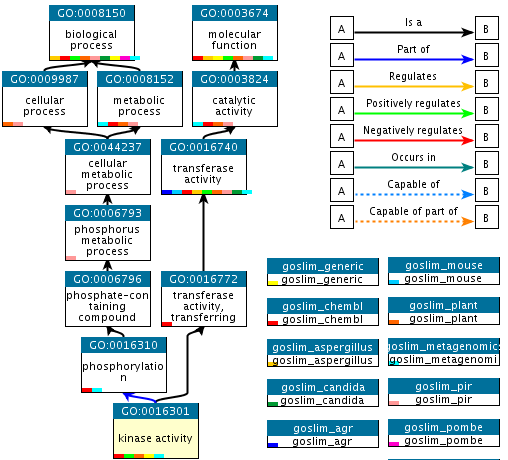
\includegraphics[width=0.8\linewidth]{img/kinase.png}
  \caption{Struktura ontologije\\ \footnotesize (preuzeto sa \parencite{go_veb})}
  \label{fig:kinase}
\end{figure}

Vremenom se GO ontologija proširuje novim tipovima relacija koje su van okvira
ovog rada.  Svaka relacija ima strogo definisana pravila kompozicije koja
omogućavaju automatsko rezonovanje. Na primer, relacija \keyword{is\_a}
ima svojstvo tranzitivnosti \parencite{is_a} prikazano Slikom \ref{fig:is_a}, a
siže pravila rezonovanja (nad relacijama) prikazan je na Slici
\ref{fig:relations}.

\lstset{
  basicstyle=\ttfamily, mathescape,
  numbers=none
}

\begin{figure}[h!]
  \centering
\begin{lstlisting}[basicstyle=\normalfont]
         A is_a    B  $\wedge$   B is_a C  $\implies$    A is_a    C           
         A part_of B  $\wedge$   B is_a C  $\implies$    A part_of C
\end{lstlisting}
\caption{Tranzitivnost relacije \keyword{is\_a} i uticaj na relaciju \keyword{part\_of}}
  \label{fig:is_a}
\end{figure}


Jedan od najčešće korišćenih formata je  ravni \file{.obo} format, a pored njega
su u upotrebi \file{RDF/XML} i \file{OWL} formati.  Poslednja dva formata
namenjena su automatskom rezonovanju unutar specijalizovanih softvera i upitnih
jezika (\textit{protégé, SPARQL, ...}).

\begin{figure}[h!]
  \centering
  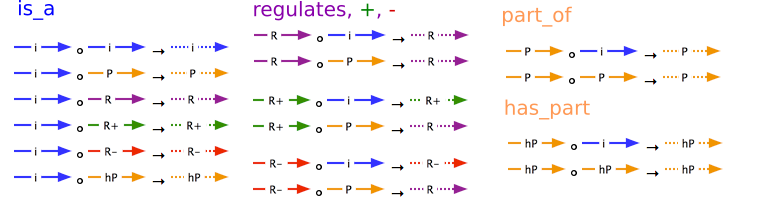
\includegraphics[scale=0.545]{relations.png}
  \caption{Pravila rezonovanja (isprekidane relacije su rezultat). \\ Elementi slike su preuzeti sa \parencite{go_veb}.}
  \label{fig:relations}
\end{figure}


\subsection{Molekulska funkcija}
\label{MF}

Funkcija genskog produkta predstavlja posao koji on obavlja ili osobinu koju on ima.
Razmotrimo narednu analogiju \parencite{go_mf}.  U kompaniji radnik (genski produkt) ima titulu
(ime genskog produkta) i vrši poslove odnosno obavlja funkcije (molekulska
funkcija) zarad izvršavanja nekog cilja tj. zadatka (biološki proces). Na
primer, funkcije vozača bile bi upravljanje volanom, stiskanje kvačila,
utovarivanje prtljaga itd, ali ne bi bilo korektno reći da je funkcija vozača
"vozačka funkcija", jer se zavisno od firme ili prevoznog sredstva menja skup
radnji koje vozač obavlja. Na primer, vozač hidrauličnog bagera neće
utovarivati prtljag ali će zato upravljati kašikom ili rotirati kabinu.

Najbitnije karakteristike molekulske funkcije su \parencite{go_mf}:
\begin{itemize}
  \item MF nije specifična za jedan genski produkt već važi za sve organizme. Dakle, ne treba mešati MF sa imenom genskog produkta.
  \item MF nije biološki proces jer se BP sastoji od nekoliko MF-ja.
  \item Granularnost staje na nivou molekula. MF ne opisuje reakcije na nivou
    atoma. Ako se reakcija može izvršavati na nekoliko načina, onda za svaki od njih
    postoji poseban MF-termin.
\end{itemize}

Postoji nekoliko standardnih definicija i šablon naziva koji se pripisuju genskom
produktu $x$ (ili nekom enzimu) \parencite{go_mf}:
\begin{itemize}
  \item \ikeyword{$x$ binding} - interaguje selektivno i nekovalentno sa $x$
  \item \ikeyword{<enzyme> activity} - katalizuje reakciju (reakcija katalizovan od strane enzima)
  \item \ikeyword{$x$ receptor activity} - vezuje se sa $x$ zarad incijacije neke ćelijske aktivnosti
  \item \ikeyword{$x$ transporter activity} - omogućava direktno pomeranje $x$ u ćeliju, iz ćelije, unutar ćelije ili između ćelija
\end{itemize}

Osim korenskog čvora MF i \ikeyword{$x$ binding} termina svi ostali MF-termini sadrže sufiks \textit{activity}.
Ovo je uvedeno iz filozofskih razloga jer za razliku od entiteta, MF-termini predstavljaju događaje, procese ili aktivnosti \parencite{go_mf}.

MF-termini takođe imaju prepoznatljiv standardni sinonim za \ikeyword{$x$ binding} \parencite{go_mf}:
\begin{itemize}
  \item \ikeyword{$x$ receptor ligand}
  \item \ikeyword{$x$ <name> binding}
\end{itemize}


\section{UniProtKB/Swiss-Prot}
\label{svis-prot}

\keyword{\uniprot} skraćeno od \textit{Universal Protein Resource} je konzorcijum
nastao 2002. izmedju tri organizacije: Evropski Bioinformatički
Institut (\textit{EBI}), Švajcarski Institut za Bioinformatiku (\textit{SIB}) i Resurs
Proteinskih Informacija (\textit{PIR}).  


\uniprot obuhvata nekoliko baza i podbaza sa striktno definisanim tokom
informacija Slika \ref{fig:uniprot_overview}. Od prikazanih najbitnija je baza
\keyword{\uniprotkb} \en{UniProt Knowledge Base} sačinjena od 2 podbaze.

\begin{figure}[h!]
  \centering
  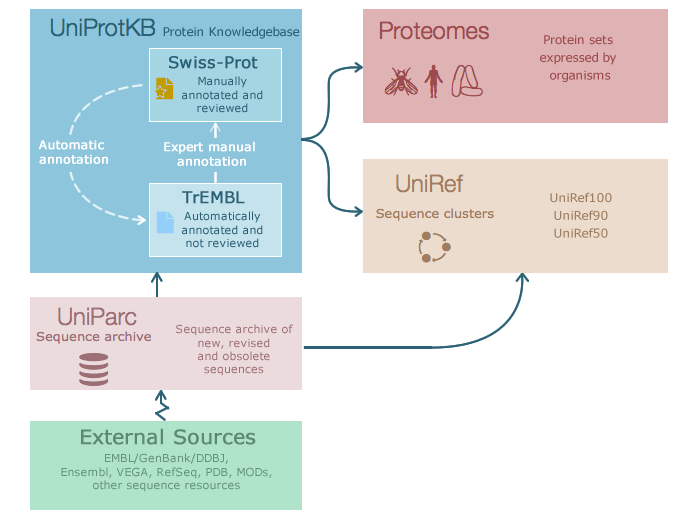
\includegraphics[width=0.8\linewidth]{uniprot_overview.png}
  \caption{Šematski prikaz povezanosti \uniprot baze\\ \footnotesize (preuzeto sa \parencite{uniprot_veb})}
  \label{fig:uniprot_overview}
\end{figure}


\begin{enumerate}
  \item \keyword{\swissprot}  sadrži visoko kvalitetne anotacije
    \keyword{neredundantnih} (termin je definisan u narednom nabrajanju,
    stavka \ref{red}) proteinskih sekvenci.  Informacije o sekvenci su dobijene
    iz postojeće literature, a automatski predviđene anotacije su ručno
    proverene i verifikovane od strane biokuratora (stručnjaci koji se brinu da
    podaci koji postanu deo baze \swissprot budu kvalitetni).  Kao baza
    podataka, \swissprot postoji preko 30 godina.

  \item \trembl \en{Translated EMBL} je nadskup sekvenci iz baze \swissprot
    dobijen prevođenjem sekvenci iz baze \textit{EMBL} (ali i sa drugih
    resursa). Automatskom računarskom analizom sekvence su anotirane funkcijom
    i osobinama, ali zbog obimne količine sekvenci ti rezultati još nisu ručno
    provereni.  Ove sekvence su \keyword{redundantne}, a njihova obimnost posledica je
    masovne primene \textit{NGS} tehnologija. U februaru 2018. god baza \trembl je sadržala
    107 627 435 sekvenci što je oko 200 puta više u poređenju sa 556 568 ručno
    proverenih sekvenci iz baze \swissprot. Sve nove sekvence prvo ulaze u sastav
    \trembl da bi ručnom proverom napredovale u \swissprot što se ogleda na
    Slici \ref{fig:uniprot_overview}.
\end{enumerate}





Distribucije baze \swissprot dostupne su u nekoliko tekstualnih formata: ravna
datoteka \en{flat file}, \textit{XML} i \textit{RDF/XML}.  Zbog
standardizacije, ravni tekstualni format prati \textit{EMBL-Bank} ravni format
\parencite{svisprot2003}.  Unos u bazu se zove \keyword{slog} \en{record} i
sadrži sve informacije vezane za jedan protein.  Jedan slog predstavljen u
formatu ravne datoteke ilustrovan je uprošćenim prikazom  na Slici
\ref{fig:slog}.  Ključne informacije koje čine slog i osobine baze \swissprot su:

\lstset{ 
  basicstyle=\fontsize{8}{10}\selectfont\ttfamily,        % the size of the fonts that are used for the code
  captionpos=b,                    % sets the caption-position to bottom
  commentstyle=\color{mygreen},    % comment style
  deletekeywords={...},            % if you want to delete keywords from the given language
  escapeinside={\%*}{*)},          % if you want to add LaTeX within your code
  extendedchars=true,              % does not work with UTF-8
  keywordstyle=\color{blue},       % keyword styli
  % language=Octave,                 % the language of the code
  morekeywords={ID, AC, PE, KW, GO, SQ}, % if you want to add more keywords to the set
  numbers=left,                    % where to put the line-numbers; 
  numbersep=5pt,                   % how far the line-numbers are from the code
  numberstyle=\color{mygray}, % the style that is used for the line-numbers
  % rulecolor=\color{black},         % if not set, the frame-color may be changed on line-breaks within not-black text (e.g. comments (green here))
  showstringspaces=false,          % underline spaces within strings only
}

\begin{figure}[h!]

\begin{lstlisting}
ID   ACSA_DROME              Reviewed;         670 AA.  | ime sloga, info
AC   Q9VP61; Q24226; Q8IH30; Q9VP60;                    | identifikacija
DT   19-SEP-2003, integrated into UniProtKB/Swiss-Prot. | ulazak u Svis-Prot
DT   01-MAY-2000, sequence version 1.                   | ulazak u TrEMBL
DT   25-OCT-2017, entry version 116.                    | poslednje 
                                                          osvezavanje sloga
\end{lstlisting}
\begin{lstlisting}[firstnumber=7,   basicstyle=\fontsize{8}{10}\selectfont\ttfamily\color{gray}]
DE   RecName: Full=Acetyl-coenzyme A synthetase;        |
DE            EC=6.2.1.1;                               |
DE   AltName: Full=Acetyl-CoA synthetase;               |
DE            Short=ACS;                                |
GN   Name=AcCoAS; ORFNames=CG9390;                      |
OS   Drosophila melanogaster (Fruit fly).               | Taksonomija
OC   Eukaryota; Metazoa; Ecdysozoa; Arthropoda; Hexap...|
OC   Pterygota; Neoptera; Holometabola; Diptera; Brac...|
OC   Ephydroidea; Drosophilidae; Drosophila; Sophopho...|
OX   NCBI_TaxID=7227 {ECO:0000312|EMBL:AAL90278.1};     |
                                                        
RN   [1] {ECO:0000305}                                  | Prva referenca
RP   NUCLEOTIDE SEQUENCE (ISOFORM B).                   | 
RA   Russell S.R., Heimbeck G.M., Carpenter A.T., Ash...| Autori
RT   "A Drosophila melanogaster acetyl-CoA-synthetase...| Naslov
RL   Submitted (NOV-1994) to the EMBL/GenBank/DDBJ da...|
RN   [2]                                                | Druga referenca              
...                                                     
CC   -!- FUNCTION: Activates acetate so that it can b...| Komentari
CC       synthesis or for energy generation.            |
CC       {ECO:0000250|UniProtKB:Q9NR19}.                |
CC   -!- CATALYTIC ACTIVITY: ATP + acetate + CoA = AM...|
...                                                     
\end{lstlisting}
\begin{lstlisting}[firstnumber=30]
DR   EMBL; Z46786; CAA86738.1; ALT_SEQ; mRNA.           | reference ka
DR   EMBL; AE014296; AAF51695.2; -; Genomic_DNA.        | drugim bazama 
...                                                     | (dbxref)
DR   ExpressionAtlas; Q9VP61; differential.             |
DR   Genevisible; Q9VP61; DM.                           |
DR   GO; GO:0005737; C:cytoplasm; IEA:UniProtKB-SubCell.| GO-termin <----
DR   GO; GO:0003987; F:acetate-CoA ligase activity; I...| GO-termin <----
...                                                     |
\end{lstlisting}
\begin{lstlisting}[firstnumber=38]
PE   2: Evidence at transcript level;
KW   Alternative splicing; ATP-binding; Complete proteome; Cytoplasm; 
KW   Ligase; Nucleotide-binding; Reference proteome.                  
FT   CHAIN         1    670       Acetyl-coenzyme A synthetase.
FT                                /FTId=PRO_0000208425.
FT   VAR_SEQ       1    146       Missing (in isoform B).
FT                                {ECO:0000303|PubMed:12537569}.
FT                                /FTId=VSP_008310.
FT   CONFLICT    227    227       C -> S (in Ref. 1; CAA86738).
FT                                {ECO:0000305}.
SQ   SEQUENCE   670 AA;  75960 MW;  CE24364755CDBFFC CRC64;
     MPAEKSIYDP NPAISQNAYI SSFEEYQKFY QESLDNPAEF WSRVAKQFHW ETPADQDKFL
...
     KKMVRERIGP FAMPDVIQNA PGLPKTRSGK IMRRVLRKIA VNDRNVGDTS TLADEQIVEQ
     LFANRPVEAK
//  <--- oznacava kraj sloga
\end{lstlisting}
\caption{Uprošćen primer sloga, preuzet iz ravne datoteke \file{uniprot\_sport.data} \footnotesize (preuzeto sa FTP servera \cite{sprot})  }
\label{fig:slog}
\end{figure}


\begin{enumerate}
  \item Ime sloga (\keyword{ID}) \en{entry name} je mnemonički zapis koji kodira
    taksonomske informacije o genu i proteinu. ID je podložan promenama 
    i ne može se koristiti kao identifikator \parencite{www_uniprot}.
  \item Identifikacioni broj (\keyword{AC}) \en{accession number} deli se u dve
    vrste.  Prvi u listi identifikatora naziva se \keyword{primarni} i služi da
    jednoznačno odredi slog. Ostatak identifikatora čine tzv.
    \keyword{sekundarani AC} i nastaju iz dva moguća razloga \parencite{svisprot2003, www_uniprot}:
    \begin{itemize}
      \item Unifikacija postojećih proteina u jedan novi slog. 
      \item Specijalizacija jednog proteina u više različitih.
    \end{itemize}
    U oba slučaja stari (primarni) AC se zadržava kao sekundarni AC u novom slogu.

  \item Za razliku od \textit{TrEMBL}, anotacije GO-terminima u bazi \swissprot
    se ručno proveravaju \parencite{www_uniprot}.

  \item \keyword{Ključne reči} (\keyword{KW}) \en{keywords} opisuju
    hijerarhisku strukturu kontrolisanog vokabulara \en{controlled vocabulary,
    CV} namenjenog opisivanju funkcije proteina. Postoji 10 kategorija ključnih
    reči od kojih je za naše istraživanje bitna "Molekulska funkcija"
    \parencite{svisprot2003}.  Za razliku od GO čiji ideal je opis svih genskih
    produkta svih vrsta, ključne reči prilagođene su opisivanju sadržaja
    isključivo baze \swissprot \parencite{www_uniprot}.

  \item Sekvenca (\keyword{SQ}) još je poznata je kao \keyword{kanonska}
    \en{canonical} sekvenca. Kanonska sekvenca predstavlja konsenzus sekvencu
    produkta (protein) gena jedne vrste organizma.  \keyword{FT} linije sadrže
    različite osobine kanonske sekvence uključujući i razlike u odnosu na
    proteinske izoforme\footnote{Proteinska izoforma je alternativni oblik sekvence
    nastao usled: alternativnog splajsovanja, upotrebe više promotera,
  alternativnih start kodona ili alternativnih okvira čitanja.}.  U
  našoj analizi korišćena je isključivo kanonska sekvenca. Detaljan opis
  pravila za utvrđivanje kanonske sekvence može se naći na \cite{www_uniprot}.

  \item
    \label{red}
    \swissprot je \keyword{minimalno redundantna} u smislu da svi proteini
    kodirani jednim genom, jedne vrste bivaju predstavljeni jednim slogom. Sve
    proteinske izoforme su grupisane pod jedan slog i jednu kanonsku sekvencu \parencite{nonRedundant}.

  \item Nivo pouzdanosti postojanja proteina (\keyword{PE}) \en{Protein existance}
    označava vrstu dokaza o postojanju proteina (Slika \ref{fig:PE}). Moguće
    vrednosti sortirane opadajuće po pouzdanosti su: potvrđeno na nivou
    proteina, potvrđeno na nivou RNK, zaključeno iz homologije, predviđen i
    nesiguran. 

  \clearpage


  \item
    Baza \swissprot takđe vrši predikcije neuređenih regiona koristeći \textit{DISOPRED2}
    i \textit{CLADIST} prediktore. \parencite{Meng_c2017}. Međutim, ove informacije
    postale su irelevantne pojavom baza neuređenja \textit{MobiDB}\parencite{Piovesan2017} i \textit{D2P2}\parencite{Oates2012}.

  \item Zanimljiva zapažanja iz globalne statistike o bazi \swissprot \cite{uniprot}:
    \begin{itemize}
      \item Većina proteina ima dužinu između 100 i 500 AK.
      \item Dokaz postojanja za oko $70\%$ proteina dobijen je iz homologije (Slika \ref{fig:PE}).
      \item Zastupljeno je preko 1000 različitih organizama, ipak
        $90\%$ proteina pripada malom broju organizama.
    \end{itemize}
      


\end{enumerate}

\begin{figure}[h!]
  \centering
  \hspace*{-0.2cm} 
  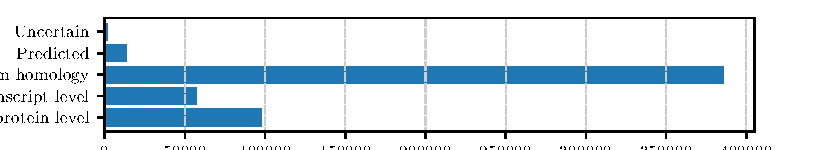
\includegraphics[]{plots/PE.pdf}
  \caption{Histogram nivoa pouzdanosti postojanja proteina iz baze \swissprot}
  \label{fig:PE}
\end{figure}

% \section{
%
% Baza proteinskog neuređenja \en{Database of protein Disorder (DisProt)}
%
% \section{D2P2 i MobiDB}
%
% Baze predviđenog neuređenja proteinskih sekvenci















\chapter{Podaci i metode} % Main chapter title

\label{Podaci i metode} % For referencing 

Cilj rada je ispitivanje veze između molekulske funkcije proteina i njegove
(ne)ure- đenosti tj. da li molekulska funkcija zavisi više od uređenosti ili
neuređenosti. Istraživanje je motivisano radom\parencite{Xie2007}. Navedeni rad
je prvi u seriji od tri rada i bavi se prvenstveno biološkim procesima i
molekulskim funkcijama.  U nastavku teksta pod terminima \keyword{originalni}
rad, autori, podaci, metode i slično podrazumevaćemo navedeni rad, njegove
autore, metode, podatke itd.

Najveća razlika u pristupu između originalnog i ovog istraživanja je što su
originalni rezultati izraženi u terminima \keyword{ključnih reči} dok su ovde
rezultati izraženi u \keyword{GO terminima}. Oba pristupa proizvode listu
funkcija koje više obuhvataju (ne)uređene proteine, ali GO termini zbog
granularnosti se prirodnije predstavljaju grafovski i sadrže mnogo više
funkcija. Jedan od rezultata ovog istraživanja predstavlja poređenje ova dva
pristupa.


\section {Podaci}

Za metode koje prezentujemo potrebne su tri vrste informacija:
\begin{enumerate}
  \item Što više različitih proteina
  \item Pouzdana anotacija funkcija
  \item Informacije o funkcijama, prvenstveno međurelacije (međurelacije između\\ funkcija su bitne  ako ih je potrebno grupisati)
\end{enumerate}


\subsection{Podaci iz originalnog rada}

U originalnom radu \parencite{Xie2007} korišćena je  baza podataka 
\keyword{\swissprot} (Poglavlje \ref{svis-prot}), verzija 48 iz 2005.
Verzija 48 ima 201 560 proteina od kojih 196 326 imaju dužinu preko 40
aminokiselina (što je potrebno zbog Definicije \ref{pdis_def} u nastavku). Funkcije
pridružene proteinima izražene su \keyword{kontrolisanim vokabularom}
\en{controlled vocabulary} koga čine takozvane \textit{UniProtKB} \keyword{ključne reči}
\en{keywords}. U verziji 48, UniProtKB sadrži 874 ključnih reči.  Zbog
statističke značajnosti posmatrane su one ključne reči kojima je bilo anotirano
barem 20 proteina, tj. 710 ključnih reči.

Kao što je pomenuto u Poglavlju \ref{svis-prot}, kanonske sekvence (proteini) u \swissprot
bazi podataka nisu redundantne u smislu da jedan unos u bazi podataka predstavlja produkt
jednog gena iz jedne vrste organizma. Međutim, za analizu funkcija
\swissprot \keyword{jeste statistički redundantna} \parencite{Xie2007} jer
sadrže veliku količinu \keyword{homologih} proteina (prvenstveno ortologa).
Zbog statističke redundantnosti originalni autori su izvršili klasterovanje \swissprot
proteina u \keyword{proteinske familije} dobivši 27 217 familija. Posledica
klasterovanja je da svaki protein dobija težinu kojom doprinosi daljoj analizi.
Težina svakog proteina u preseku klastera sa datom funkcijom je obrnuto
proporcionalna veličini preseka tako da je zbir težina svih proteina jednaka
veličini preseka.

% \textbf{komentar:} \\
% Ono što autori nisu elaborirali jeste da početni uslov od minimum 20 proteina
% po ključnoj reči možda nije dovoljan. Ako pretpostavimo zarad ilustracije
% normalnu raspodelu veličina klastera proteina, očekivali bi da klaster najčešće
% sadrži 7 proteina. Dakle iako je 50 proteina pridruženo nekoj funkciji ona
% verovatno ima pridruženih svega 7 familija proteina. Kako familija sadrži
% proteine pod pretpostavkom istog evolutivnog porekla njihova funkcija bi
% trebalo da je slična pa se onda postavlja pitanje da li je 7 familija dovoljno
% da bi se razmatrala data ključna reč. Ovo je primarno kritika za ključne reči
% jer one obično predstavljaju opšte pojmove.
%
% Sa druge strane za usko specijalizovane pojmove bila bi dovoljna jedna familija
% proteina jer bi ona predstavljala sve razne homologe (TODO Burkhard Rost,
% Termofili)

\subsection{Podaci korišćeni u ovom istraživanju}

Ugledom na \keyword{CASP} takmičenja, \keyword{CAFA} \en{Critical Assessment of
Functional Annotation} takmičenje pokrenuto je zarad objektivnog ocenjivanja
prediktora funkcije proteina i usmeravanja budućeg razvoja ove oblasti
\parencite{CAFA}.  U ovom radu korišćen je trening skup proteina preuzet sa
\keyword{CAFA3} takmičenja, održanog 2017. Trening skupovi su podaci na osnovu
kojih prediktor uči, pa shodno tome ovaj skup treba da predstavlja dobar uzorak
proteina odnosno njihovih funkcija.

CAFA3 trening skup (u nastavku samo CAFA3 skup ili CAFA3 podaci) je podskup \swissprot baze (iz 2016.) koji
uključuje proteine iz model organizama: \textit{Human, Mouse, Rat, S.
cerevisiae, S. pombe, E. coli, A. thaliana, Dictyostelium discoideum,
Zebrafish, Bacillus cereus} sa izuzetokm sekvenci \textit{Drosophila} i \textit{Candida}
koje su preuzete iz svojih genomskih baza podataka, respektivno.
Slika \ref{fig:sp_vs_cafa3} pruža detaljan taksonomski uvid o poreklu CAFA3 proteina.
Na primer, \swissprot baza sadrži oko 20 000 ljudskih (\textit{Homo})
proteinskih sekvenci dok CAFA3 podskup sadrži malo manje od 15 000.  Vrste
koje doprinose sa manje od 100 proteina nisu prikazane radi kompaktnosti.

\begin{figure}[th]
\centering
\hspace*{-3.0cm} 
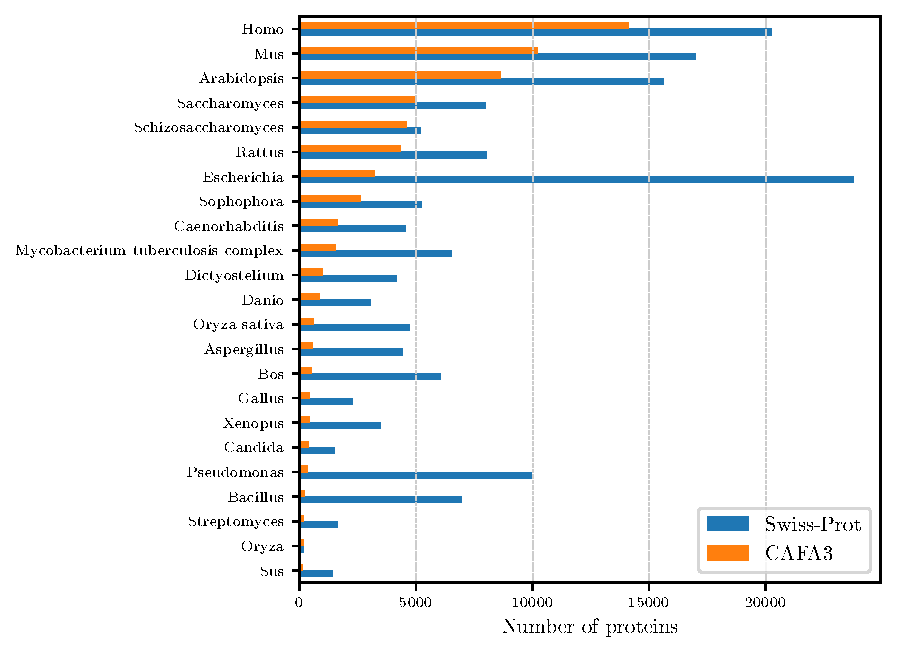
\includegraphics[]{plots/sp_vs_cafa3}
% \decoRule
\caption{Taksonomsko poreklo CAFA3 proteina. \\ \footnotesize 
}
\label{fig:sp_vs_cafa3}
\end{figure}

Za razliku od proteina u \swissprot bazi čije je postojanje pretežno utvrđeno
iz homologije, $74\%$ proteina iz CAFA3 podskupa identifikovani su na nivou
nivou proteina što je najveći stupanj sigurnosti da proteini zaista postoji. Na
Slici \ref{fig:cafa3_pe} ilustrovana je razlika u odnosu na pouzdanost
postojanja proteina. 



\begin{figure}[th]
\centering
\hspace*{-2.5cm} 
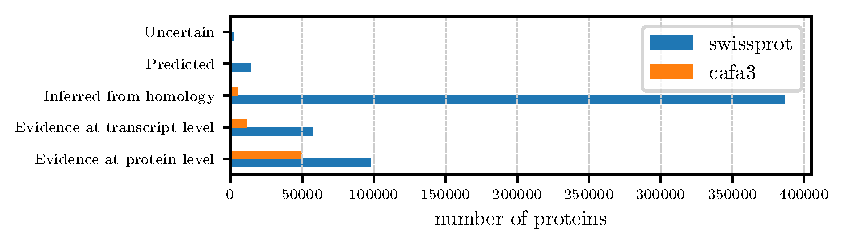
\includegraphics[]{plots/cafa3_pe}
% \decoRule
\caption{Razlika izmedju pouzdanosti postojanja proteina iz \\ \swissprot baze i njenog CAFA3 podskupa. }
\label{fig:cafa3_pe}
\end{figure}


Važno je naglasiti da je dalja analiza izvršena pod pretpostavkom da CAFA3 skup
nije statistički redundantan, što znači da klasterovanje u proteinske familije
nije potrebno.  Isključivanje ove pretpostavke bi dovelo do komplikovanijih
računarskih metoda za analizu što je van opsega ovog rada.



% Iako ovaj pristup potencijalno proizvodi skup koji je \keyword{statisički
% redundantan} u našoj analizi smo pretpostavili da to nije slučaj jer je čin
% klasterovanja veoma računarski zahtevan, a nismo ubeđeni da je neophodan za
% ovaj konkretan skup. Iz tog razloga u daljoj analizi predstavljamo uprošćenu
% verziju formule koja ne uračunva težinu pojedinačnog proteina.

\swissprot proteini su kodirani jednim karakterom koristeći \keyword{IUPAC}
kodove.  U podacima javljaju se sekvence sa  21. i 22. aminokiselinom ('U' i 'O')
kao i  višeznačne oznake: 'B', 'J', 'X' i 'Z'.  Ovakve sekvence nisu podržane od
strane VSL2b prediktora i za nas predstavljaju nevalidne proteinske sekvence. Pod
\keyword{validnom proteinskom sekvencom} smatraćemo sekvencu koja je validan
ulaz za VSL2b, tj. čini je azbuka od 20 standardnih aminokiselina i
ima minimalnu dužinu 9 AK.

CAFA3 Podaci se sastoje od dve datoteke:
\begin{enumerate}
  \item \file{uniprot\_sprot\_exp.fasta}  sadrži 66 841 protein od kojih 66 599
    za našu analizu predstavljaju validnu proteinsku sekvencu. Od preostalih
    proteina 66 063 ima dužinu veću ili jednaku od 40 aminokiselina.
  \item \file{uniprot\_sprot\_exp.txt} proteinima pridružuje funkcije u obliku 
    \keyword{GO termina}. Zastupljeni su termini iz sva tri imenska prostora:
    16 117 ćelijskih komponenti, 5 966 molekulskih funkcija i 16 117 bioloških
    procesa. Jednom proteinu može biti pridruženo više GO termina i obrnuto.
\end{enumerate}

Analiza u ovom radu je primarno orijentisna ka korišćenju GO termina za opis
funkcije što je razlikuje od originalnog pristupa korišćenja ključnih reči.
Analiza GO termina zahteva poznavanje prvenstveno \textit{is\_a} roditeljske
veze između termina. Takođe, tokom istraživanja bile su nam potrebne i ostale
informacije o terminima. Pomenute informacije dobili smo iz datoteke
\file{go.obo} \cite{go_obo} verzije 01.12.2017.

Odnos tj. mapiranje između ključnih reči i GO termina dostupno je sa dva izvora:
\begin{itemize}
  \item \file{keywlist.txt}\cite{keywlist_txt} verzija 20.12.2017 sadrži
    informacije o 1188 ključnih reči od kojih 195 pripada kategoriji
    \keyword{Molekulskih funkcija}. Više o mapiranju biće
    izloženo u Potpoglavlju \ref{kw2go_mapiranje}.
  \item \file{uniprotkb\_kw2go}\cite{uniprotkb_kw2go} sadrži samo mapiranja a
    generiše ih \keyword{GOA projekat} \parencite{Barrell2009}. 
\end{itemize}

U ovom radu korišćena je isključivo \file{keywlist.txt} datoteka. Iako je
datoteka \\ \file{uniprot\_kw2go} sadržala veći broj mapiranja, unosila je
nepoželjnu višeznačnost.

Pošto je originalni rad iz 2007. godine, postoje razlike u broju proteina,
anotacijama ključnih reči, broju ključnih reči ali i primarnoj strukturi proteinskih
sekvenci.  Radi procene uticaja navedenih razlika na rezultat, odlučeno je da se
analiza prvo ponovi originalnim pristupom, koristeći vokabular ključnih reči.
Iz tog razloga, CAFA3 podaci nisu mogli da se posmatraju kao crne kutije, već
je bilo neophodno mapirati ih nazad na \swissprot proteine čije su anotacije 
ključnim rečima poznate. Ovaj korak objedinjavanja baza podataka opisan je u
Potpoglavlju \ref{objedinjavanje}. Dobijene anotacije ključnim rečima takođe su
iskorišćene za proveru validnosti mapiranja ključnih reči na GO termine.
Mapiranja su detaljno opisana u Potpoglavlju \ref{kw2go_mapiranje}



\section {Metod}


Pod \keyword{idealnim slučajem},
pretpostavimo da za proizvoljnu molekulsku funkciju znamo sve strukturno različite
proteine koji je obavljaju.  Da bi dali korektan odgovor  moramo da znamo kako
neuređenost pojedinačnog proteina utiče na
na njegovo ponašanje, i kako to ponašanje (tip neuređenosti) utiče na datu funkciju.
% Ova vrsta znanja nije bila dostupna 2007. osim za jako mali skup proteina.

Nažalost, ograničenja današnjih podataka i razvijenih metoda su brojna:
\begin{itemize}
  \item
    Baza eksperimentalno utvrđenih neuređenih regiona
    \textit{\keyword{DisProt}} ima svega 803 proteina sa opisanih 2167
    neuređenih regiona \parencite{Piovesan2016}.  Uz to, kvalitet navedenih
    informacija je diskutabilan zbog razlika u pouzdanosti među
    eksperimentalnim tehnikama koje su korišćene.  Najveću pouzdanost nose
    regioni koji su eksperimentalno okarakterisani sa što većim brojem
    laboratorijskih tehnika.

  \item
    Prediktori se treniraju na malom podskupu proteina iz \textit{DisProt}
    i PDB  baze. Čak i konsenzus nekoliko različitih prediktora ne daje
    dovoljno pouzdane rezultate o lokaciji neuređenog regiona.

  \item 
    Pozitivna strana je najnoviji napredak, razvoj prediktora koji direktno
    pokušavaju da predvide funkciju koju IDPr obavlja \parencite{Meng_c2017}.
  % \item Koliko nam je poznato trenutno nema prediktora koji predviđaju tip
  %   neuređenosti. Takođe, Opisivanje tipa neuređenosti predstavlja poduhvat.
  %   \begin{itemize}
  %     \item Prof. Vladimir Uverski predlaže nekoliko imena za opis različitih
  %       ponašanja neuređenih proteina \en{Folldon, Unfolldon, ...}
  %       \parencite{Uversky2017}.
  %     \item Prof. Peter Tompa je zaslužan za kreiranje 3 ontologije neuređenih
  %       regiona za bazu Disprot koji precizno modeluje tipove
  %       neuređenosti \parencite{disprot}.  .  Međutim koliko nam je poznato
  %       prediktori koji predviđaju termine ove ontologije još nisu napravljeni
  %   \end{itemize}

\end{itemize}

Jednostavna alternativa idealnom slučaju je da se pretpostavi da veći udeo neuređenih u odnosu
na uređene proteine podrazumeva da funkcija zavisi više od neuređenosti. 
% Dakle izjednačavamo uzročnost \en{causation} i \keyword{korelaciju} između funkcije i neuređenosti.
% Međutim, prvo je potrebno precizirati kada protein smatramo neuređenim.
% Definicija mora da ima biološkog smisla, da bude prilagođena
% analizi, ali pored takođe je ograničena sposobnostima i preciznošću prediktora
% koji se korist.  Više o tome u narednom Potpoglavlju \ref{naredno}.

\subsection{Predikcija neuređenosti proteina}
\label{naredno}

Originalni autori koristili su \keyword{PONDR VL3E} prediktor koji
postiže tačnost od $~87\%$ pri unakrsnoj validaciji nad uravnoteženim test
skupom.  Zbog ekonomičnosti i dostupnosti u ovom radu korišćen je noviji
prediktor druge generacije \keyword{PONDR VSL2b}.
Relevantne karakteristike VSL2b prediktora detaljno su opisane u \ref{VSL2b}.
Za potrebe analize originalni autori  uvode sledeću definiciju:

\newtheorem{mydef}{Definicija}
\begin{mydef}
\label{pdis_def}
Protein je \keyword{putativno neuređen} (najverovatnije neuređen, u daljem tekstu neuređen) engl. putatively disordered
ako sadrži bar jedan region veći ili jednak od 40 uzastopnih aminokiselina
takvih da im je predviđenu neuređenost iznad 0.5. 
\end{mydef}

Onda definišemo operator $d$ takav da za svaku proteinsku sekvencu $s_i$ važi:

\[   
  d(s_i) = 
    \begin{cases}
      1 & \text{ako je} \quad s_i \quad \keyword{neuređena}\\
      0 & \text{suprotno}
    \end{cases}
\]

Uslov ''$\ge40$'' u originalnom radu delom je posledica ograničenja VL3
prediktora koji je treniran nad skupom sekvenci sa dugim neuređenim regionima
\footnote{L označava duge regione, $\ge$ 30 AK}.
% Mi nismo u obavezi da sledimo ovo pravilo, ali ga sledimo radi upoređivanja rezultata.

\subsection{Zavisnost dužine proteina i predikcije dugačkog neuređenog regiona}

Verovatnoća da po gornjoj definiciji protein bude klasifikovan kao neuređen
raste sa porastom njegove dužine. Ovo ponašanje  utiče na statističku
značajnost rezultata.  Originalni autori predlažu narednu formulu za procenu
pomenute verovatnoće.

Neka je $S_L$ skup proteina sa dužinama iz intervala $[L-l, L+l]$\footnote{Na
primer, skup $S_{100}$ sadrži proteine iz intervala $[90, 110]$, a $S_{500}$ iz
intervala $[450, 550]$} gde je $l = 0.1 \cdot L$. Dobijamo sledeće formule:

$$ S_L = \{s_i : \quad | L -  | s_i | | \le l \quad \}, \quad   |s_i| \text{ je dužina sekvence}  $$
$$ P_L = \dfrac{ \sum_{s_i \in S_L} d(s_i)} {| S_L |}, \quad   |S_L| \text{ je kardinalnost skupa}$$

Grafik funkcije $P_L$ u zavisnosti od promenljive $L$ predstavljen je na Slici
\ref{fig:PL1}.  Glatkoća rezulatata kontroliše se veličinom $l$ koja
predstavlja prozor uprosečavanja. Kako prozor uprosečavanja raste sa porastom
dužine proteina $(l = 0.1 \cdot L)$ tako $P_L$ postaje glađa sa veličinom
promenljive $L$. Ovo je suprotno konstantnom prozoru uprosečavanja  koji je
tehnika još poznata kao \textit{rolling average} ili \textit{boxcar filter} i
predstavlja prostu vrstu konvolucije. 


\begin{figure}[th]
\centering
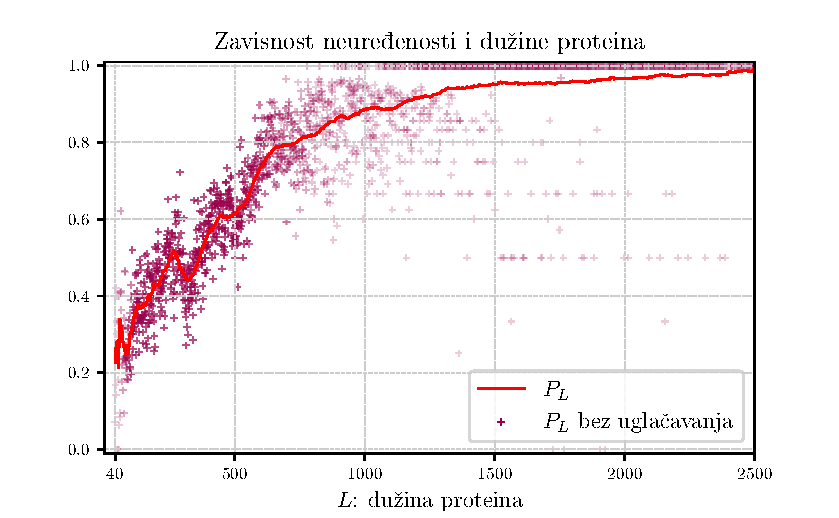
\includegraphics[]{plots/PL_F}
% \decoRule
\caption {
  Zavisnot neuređenosti i dužine CAFA3 proteina minimalne dužine 40 AK
  \footnotesize
  ($P_L$ sa prozorom uprosečavanja podrazumeva $l = 0.1L$, dok
  krstići predstavljaju diskretne vrednosti L za $l = 0$. Transparentnost krstića
  ilustruje brojnost proteina dužine $L$. Ako je krstić transparentan
  znači da sadrži manje od 100 proteina.)
}
\label{fig:PL1}
\end{figure}


Pored gore prikazanog originalnog metoda predložićemo još jedan pristup
procenjivanju veličine $P_L$.
% \keyword{Slučajno generisani} \en{random generated} proteini za procenu $P_L$.
Razmotrićemo dva modela zasnovana na slučajno generisanim proteinima. Prvi,
naivni model \keyword{uniformne verovatnoće} podrazumeva da se svaka
aminokiselina javlja sa istom verovatnoćom, odnosno $p=1/20$. U statistici je ovaj
model još poznat kao model jednakih verovatnoća \en{equiprobable model
(EPM)}.  Drugi model koji ćemo zvati slučajni ili \textit{random} model RM)  predstavlja
slučajnu promenljivu čija verovatnoća zavisi od učestalosti aminokiselina iz
CAFA3 skupa i prikazana je na Slici \ref{fig:AK_ucestalost}.
% Koristeći ova dva modela za svaki protein generisan je slučajan protein iste
% dužine koji se koristi za procenu $P_L$.
Na osnovu predstavljenih modela definisana su dva nova skupa sekvenci (EPMS i
RMS) iste kardinalnosti kao polazni CAFA3 skup, u kojima su sekvence bile istih
dužina kao u polaznom skupu. U EPMS, sekvence su generisane na osnovu uniformne
raspodele nukleotida, dok su u RMS sekvence definisane na osnovu učestalosti
aminokiselina iz CAFA3 skupa.


\begin{figure}[th]
\centering
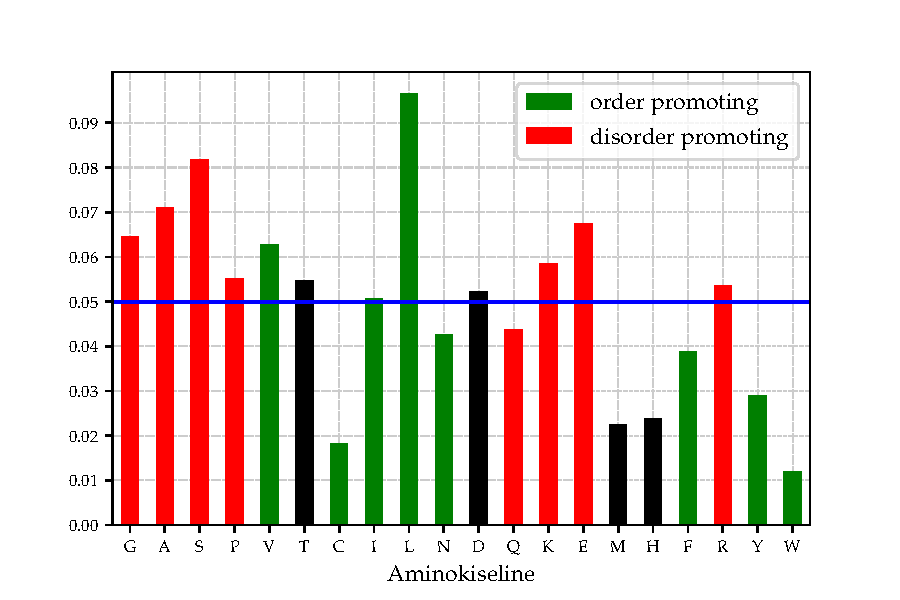
\includegraphics[]{plots/AK_ucestalost}
% \decoRule
\caption{
  Učestalost aminokiselina u CAFA3 podacima
  \\ \footnotesize
  (Učestalost prikazuje uniformni model, dok boja AK obeležava afinitet prema
  uređenosti ili neuređenosti. Aminokiseline su poređane u rastućem poretku
  od najlakše do najteže. 
}
\label{fig:AK_ucestalost}
\end{figure}

Poređenje predloženih modela sa originalnim $P_L$ prikazano je na Slici
\ref{fig:PL2}. Jasno se vidi da slučajni model predstavlja vizuelno dobru
aproksimaciju dok uniformni model znatno odstupa rastući sporije (naizgled
skoro linearno).
% Kako VSL2b prediktor prepoznaje neuređene regione na osnovu učestalosti
% aminokiselina, ovo ponašanje nije čudno jer je manja verovatnoća pojave
% aminokiselina koje promovišu neuređenost.
Zbog znatnog vizuelnog odstupanja uniformni model nije korišćen u daljoj analizi.


\begin{figure}[th]
\centering
% 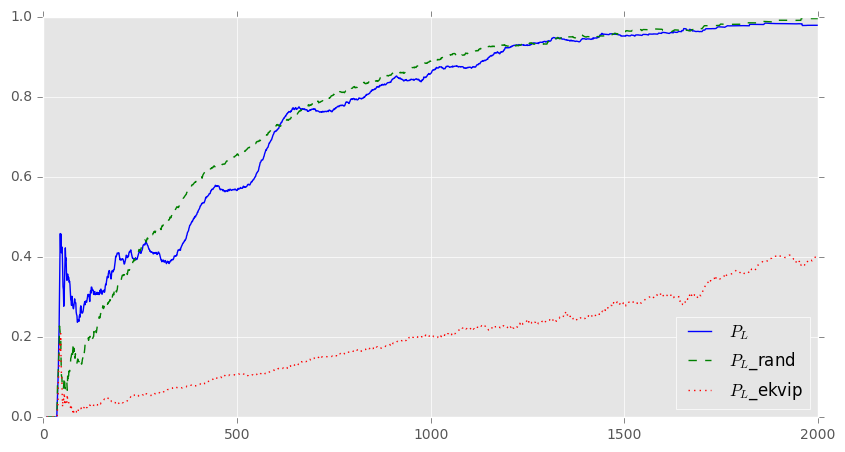
\includegraphics[scale=0.65]{Figures/PL2}
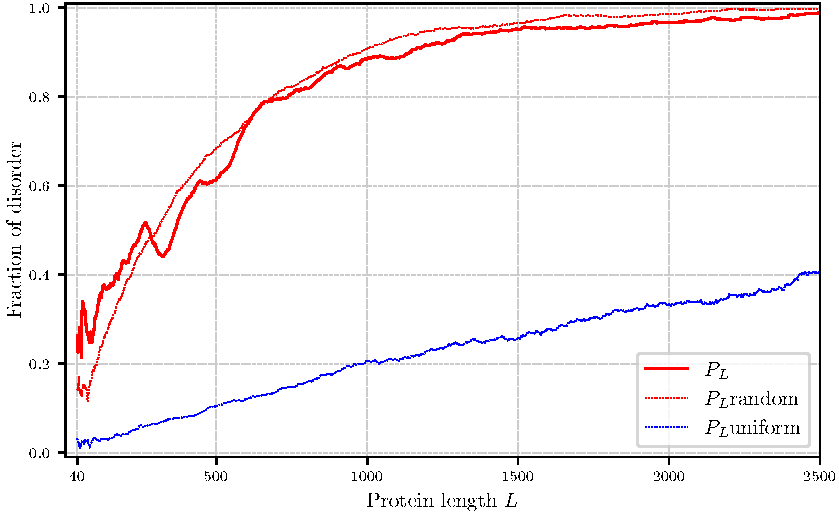
\includegraphics[]{plots/PL_F_cmp}
% \decoRule
\caption{Upoređivanje $P_L$, $P_L random$ i $P_L uniform$ modela nad CAFA3 podacima}
\label{fig:PL2}
\end{figure}


Jedno od objašnjenja zašto je uniformni model naivan i toliko odstupa od
prvobitnog metoda proizilazi iz činjenice da aminokiseline imaju inherentno
različitu učestalost u živom svetu. Naime, aminokiseline ne mogu  imati istu
verovatnoću pojavljivanja jer se  broj njihovih kodona razlikuje. Neke
aminokiseline su kodirane sa samo jednim, a druge i sa 6 kodona. Očekivano je
da veći broj kodona povećava učestalost aminokiseline i ta korelacija uz
izuzetke arginina predstavljena je Slikom \ref{fig:aminoacid}
\parencite{AKfrekvencija}.

\begin{figure}[th]
\centering
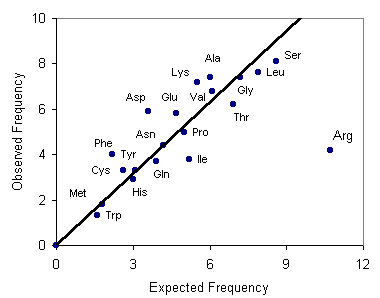
\includegraphics[scale=0.7]{aminoacid}
% \decoRule
\caption{Očekivana i izmerena učestalost aminokiselina kod kičmenjaka (preuzeto sa \cite{AA_freq_link}).  \footnotesize
  Izmerena učestalost dobijena je analizom 53 kompletno sekvencionirana proteina iz kičmenjaka \cite{King1969}.
  Očekivana učestalost kodona izračunata je kao proizvod učestalosti nukleinskih baza koje ga čine.
  Očekivana učestalost aminokiseline je zbir očekivanih učestalosti njenih kodona.
}
\label{fig:aminoacid}
\end{figure}




\clearpage
\label{ocenjivanje}
\subsection{Ocenjivanje zavisnosti funkcije od neuređenosti}

Neka je $S_j$ skup proteina koji imaju pridruženu funkciju $j$. Tada se procenat
neuređenih proteina u oznaci $F_j$ može izračunati kao:
$$F_j = \dfrac{\sum_{s_i \in S_j} d(s_i)} {|S_j|} $$



Nulta hipoteza za $F_j$ je tvrdnja da $F_j$ zavisi samo od dužine sekvence tj. $P_L$. \\
Neka je $X_L$ Bernulijeva slučajna promenljiva oblika $X_L : \begin{pmatrix} 0 & 1\\ P_L & 1-P_L \end{pmatrix}$. \\
Tada nultu hipotezu modeliramo raspodelom $Y_j$, koja za razliku od $F_j$ koristi
slučajnu promenljivu $X_L$ umesto  $d(s_i)$, odnosno:


% Nultu hiptezu koja predviđa da je rezultat $F_j$ posledica samo slučajnosti, to
% jest zavisi samo od $P_L$ opisana je preko slučajne veličine $Y_j$ gde je $X_L$
% Bernulijeva slučajna veličina sa verovatnoćom $P(X_L = 0) = P_L$ odnosno $P(X_L
% = 1) = 1-P_L$

$$ Y_j = \dfrac {\sum_{s_i \in S_j} {X_{|s_j|}}}{|S_j|}$$

Ako $F_j$ izlazi iz intervala poverenja raspodele $Y_j$ onda funkcija $j$
sadrži značajno mnogo predviđenih (ne)uređenih proteina. Preciznije,
ako je p-vrednost \en{p-value} manja od 0.05 onda je funkcija $j$ povezana sa neuređenim
proteinima, a ako je \textit{p-value} veća od 0.95 onda je funkcija $j$ povezana sa
uređenim proteinima.  Suprotno, povezanost funkcije $j$ sa (ne)uređenošću nije
statistički značajna.  

U nastavku teksta, pod neuređenošću funkcije, ključne reči ili GO termina, biće
podrazumevano da je odgovarajuća p vrednost manja od 0.05. Analogno, pod
uređenošću funkcije, ključne reči ili GO termina, biće podrazumevano da je
odgovarajuća p vrednost veća od 0.95.
% Kada se kaže da je funkcija, ključna reč ili GO termin (ne)uređen
% podrazumevaće se da je odgvorajauća p-vrednost manja od $0.05$ ili veća
% od $0.95$.

Zbog matematičkog oblika $X_L$ teško je analitički proceniti $Y_j$ pa se se
pribegava empirijskom računanju p-vrednosti. Empirijska p-vrednost određena je
tako što je za 1000 realizacija $Y_j$ izračunato očekivanje da je realizacija
$Y_j$ veća od $F_j$.

Preciznije, vektor\footnote{zamenili smo skup $S_j$ za vektor $S_j$. Ovo je
implementacioni detalj} $S_j$ sadrži $k$ proteina $S_j=\{s_1, s_2, ...
,s_{k}\}$.  Protein $s_i$ ima dužinu $L_i$ za koju je izračunata verovatnoća
$P_{L_i}$.  Tada generatorom Bernulijevih slučajnih brojeva, za svaki protein
$p_i$ na osnovu $P_{L_i}$ generišemo realizaciju $X_L$. Rezultat je vektor od
$k$ vrednosti nula ili jedan. Učestalost jedinica u rezultujućem vektoru
predstavlja prvu realizacija $Y_j$.  Postupak se ponavlja 1000 puta i broji
se koliko puta je realizacija $Y_j$ bila veća od $F_j$. Dobijeni zbir deli se
sa 1000 i rezulatat je empirijska p-vrednost.

% \begin{verbatim}
%     p = np.array( [yj>Fj for yj in Yj_1000] ).mean()
% \end{verbatim}

Originalni autori tvrde da se za veće skupove $S_j$, raspodela
$Y_j$ ponaša kao normalna. To znači da se ocena Z-skor može dobiti kao
$Z_j=(F_j-\mu_j)/\delta_j$ gde je $\mu_j$ očekivanje, a $\delta_j$ standardna
devijacija. 
% Dodatno, p-vrednost može da se aproksimira kao $1/2(1-erf(Z_j/2))$
% \footnote{$erf()$ je gausova funkcija greške,
% $erf(x)=\dfrac{2}{\sqrt{\pi}} \int_{0}^{x}  e^{-t^2} dt$ }
% ako raspodela liči na normalnu. Ovo je nekad korisno jer sa 1000 realizacija
% $Y_j$ nema dovoljnu preciznost za p vrednost manju od $1/1000=0.001$. Međutim u
% ovom radu to nije korišćeno jer su sva sortiranja (kao i u originalnom radu)
% izvršena po Z-skor oceni.




\chapter{Priprema podataka} % Main chapter title

\label{Priprema_podataka} % For referencing 

\section{Objedinjavanje starih CAFA3 i novih Svis-Prot proteina}

iz CAFA3 trening skupa izdvojeni su svi validni proteini ( dužine barem 9, i
azbukom od 20 standardnih aminokiselina). Ni u jednom trenutko ne izbacujemo
proteine manje od 40 aminokiseline jer to deo analize funkcije i nismo želeli
da ograničimo skup mogućih predikcija neuređenosti.

Informacije o Svis-Prot bazi dobijene su iz verzije 2017\_12, iz datoteke
\url{ftp://ftp.uniprot.org/pub/databases/uniprot/previous_releases/release-2017_12/knowledgebase/uniprot_sprot-only2017_12.tar.gz}.
Pomenuta verzija ima 556.196 proteina. Zbog novijeg datuma baze postoje razlike
u broju, sekvencama i  anotacijama proteina u odnosu na CAFA3 verzije proteina.

\section{}


% 
\chapter{Implementacija} % Main chapter title

\label{Implementacija} % For referencing 


%------------------------------------------------------------------------------






\chapter{Rezultati} % Main chapter title

\label{Rezultati} % For referencing 

Računarska analiza implementirana je u jeziku Pajton \en{Python} verzija 3.6.
Kompletan projekat može se naći na \textit{github} adresi \cite{projekat}. Za
potrebe projekta napravljene su dve baze podataka: relaciona baza podataka
(\textit{PostgreSQL} v9.5) i grafovska baza podataka (\textit{Neo4j} v3.1).

Od 186 MF ključnih reči koje anotiraju bar 20 proteina, 97 je statistički
značajno od čega su 53 predviđeno uređene (p<0.05), a 44 predviđeno neuređene
(p>0.95).  Od 1781 MF termina sa preko 20 pridruženih proteina (dobijeno
grupisanjem, Potpoglavnje \ref{grupisanje}), 1315 je statistički značajno od
čega su 699 predviđeno uređeni, a 616 predviđeno neuređeni.  Tabela
\ref{tab:kw_uopsteno} prikazuje razlike u odnosu na originalne rezultate.

\begin{table}[htpb]
\begin{tabular}{|r|c|c|c|}
  \hline
                     & \small originalni rezultati  & \multicolumn{2}{c|}{ novi rezultati} \\
                     & Xie2007 kw & MF kw  & MF termini                  \\
  \hline
  ukupno ($br. prot\ge20$)     & 143        & 186    & 1781                        \\
  p<0.05 (uređene)   & 37         & 53     & 699                         \\
  p>0.95 (neuređene) & 51         & 44     & 616                         \\
  \hline
\end{tabular}
  \centering
  \caption{Uopšteno poređenje rezultata}
  \label{tab:kw_uopsteno}
\end{table}

Slika \ref{fig:disorder_cmp} sadrži tri tabele predviđeno neuređenih funkcija
koje sadrže: rezultate iz originalnog rada \cite{Xie2007} (levo), nove
rezultate za MF ključne reči (sredina) i rezultate za mapirane MF termine
(desno). Sve tabele su sortirane po z-skoru opadajuće (statistička značajnost
predviđene neuređenosti opada).  Leva tabela sadrži samo 20 statistički
najznačajnije neuređenih MF ključnih reči dok je srednja ograničena na z-skor
veći od dva.  Redovi leve tabele su crveni ako se odgovarajuća ključna reč ne
nalazi u srednjoj tabeli.  Redovi srednje tabele su zeleni ako se nalaze među
prvih 20 a ključna reč se ne javlja u levoj tabeli.  Desna tabela MF termina
sadrži samo one termine koji su rezultat direktnog ili izvedenog mapiranja.
Punim strelicama prikazana su direktna mapiranja, a isprekidanim izvedena.
Nedostatak veze između srednje i desne tabele sugeriše da suprotna funkcija
nije statistički značajna, a crvena boja redova u srednjoj tabeli označava da
ni direktno ni indirektno mapiranje ne postoji.  Srednja i desna tabela pored
kolona z-skor i p vrednosti sadrže i procenat neuređenih proteina
(\text{avg\_dis}) na koji se ubuduće referišemo kao \keyword{neuređenost
funkcije}. Slike \ref{fig:disorder_cmp_ab}a, \ref{fig:disorder_cmp_ab}b
pojednostavljuju sagledavanje pojedinačnih razlika među rezultatima, međutim
zbog ograničenja formata slike neke tabele su skraćene.

Slike \ref{fig:order_cmp} i \ref{fig:order_cmp_ab}  imaju ekvivalentan format
poređenja kao i Slike \ref{fig:disorder_cmp} i \ref{fig:disorder_cmp_ab}, ali
predstavljaju sortirane uređene funkcije.



\clearpage

\begin{figure}[th]
\hspace*{-2.5cm} 
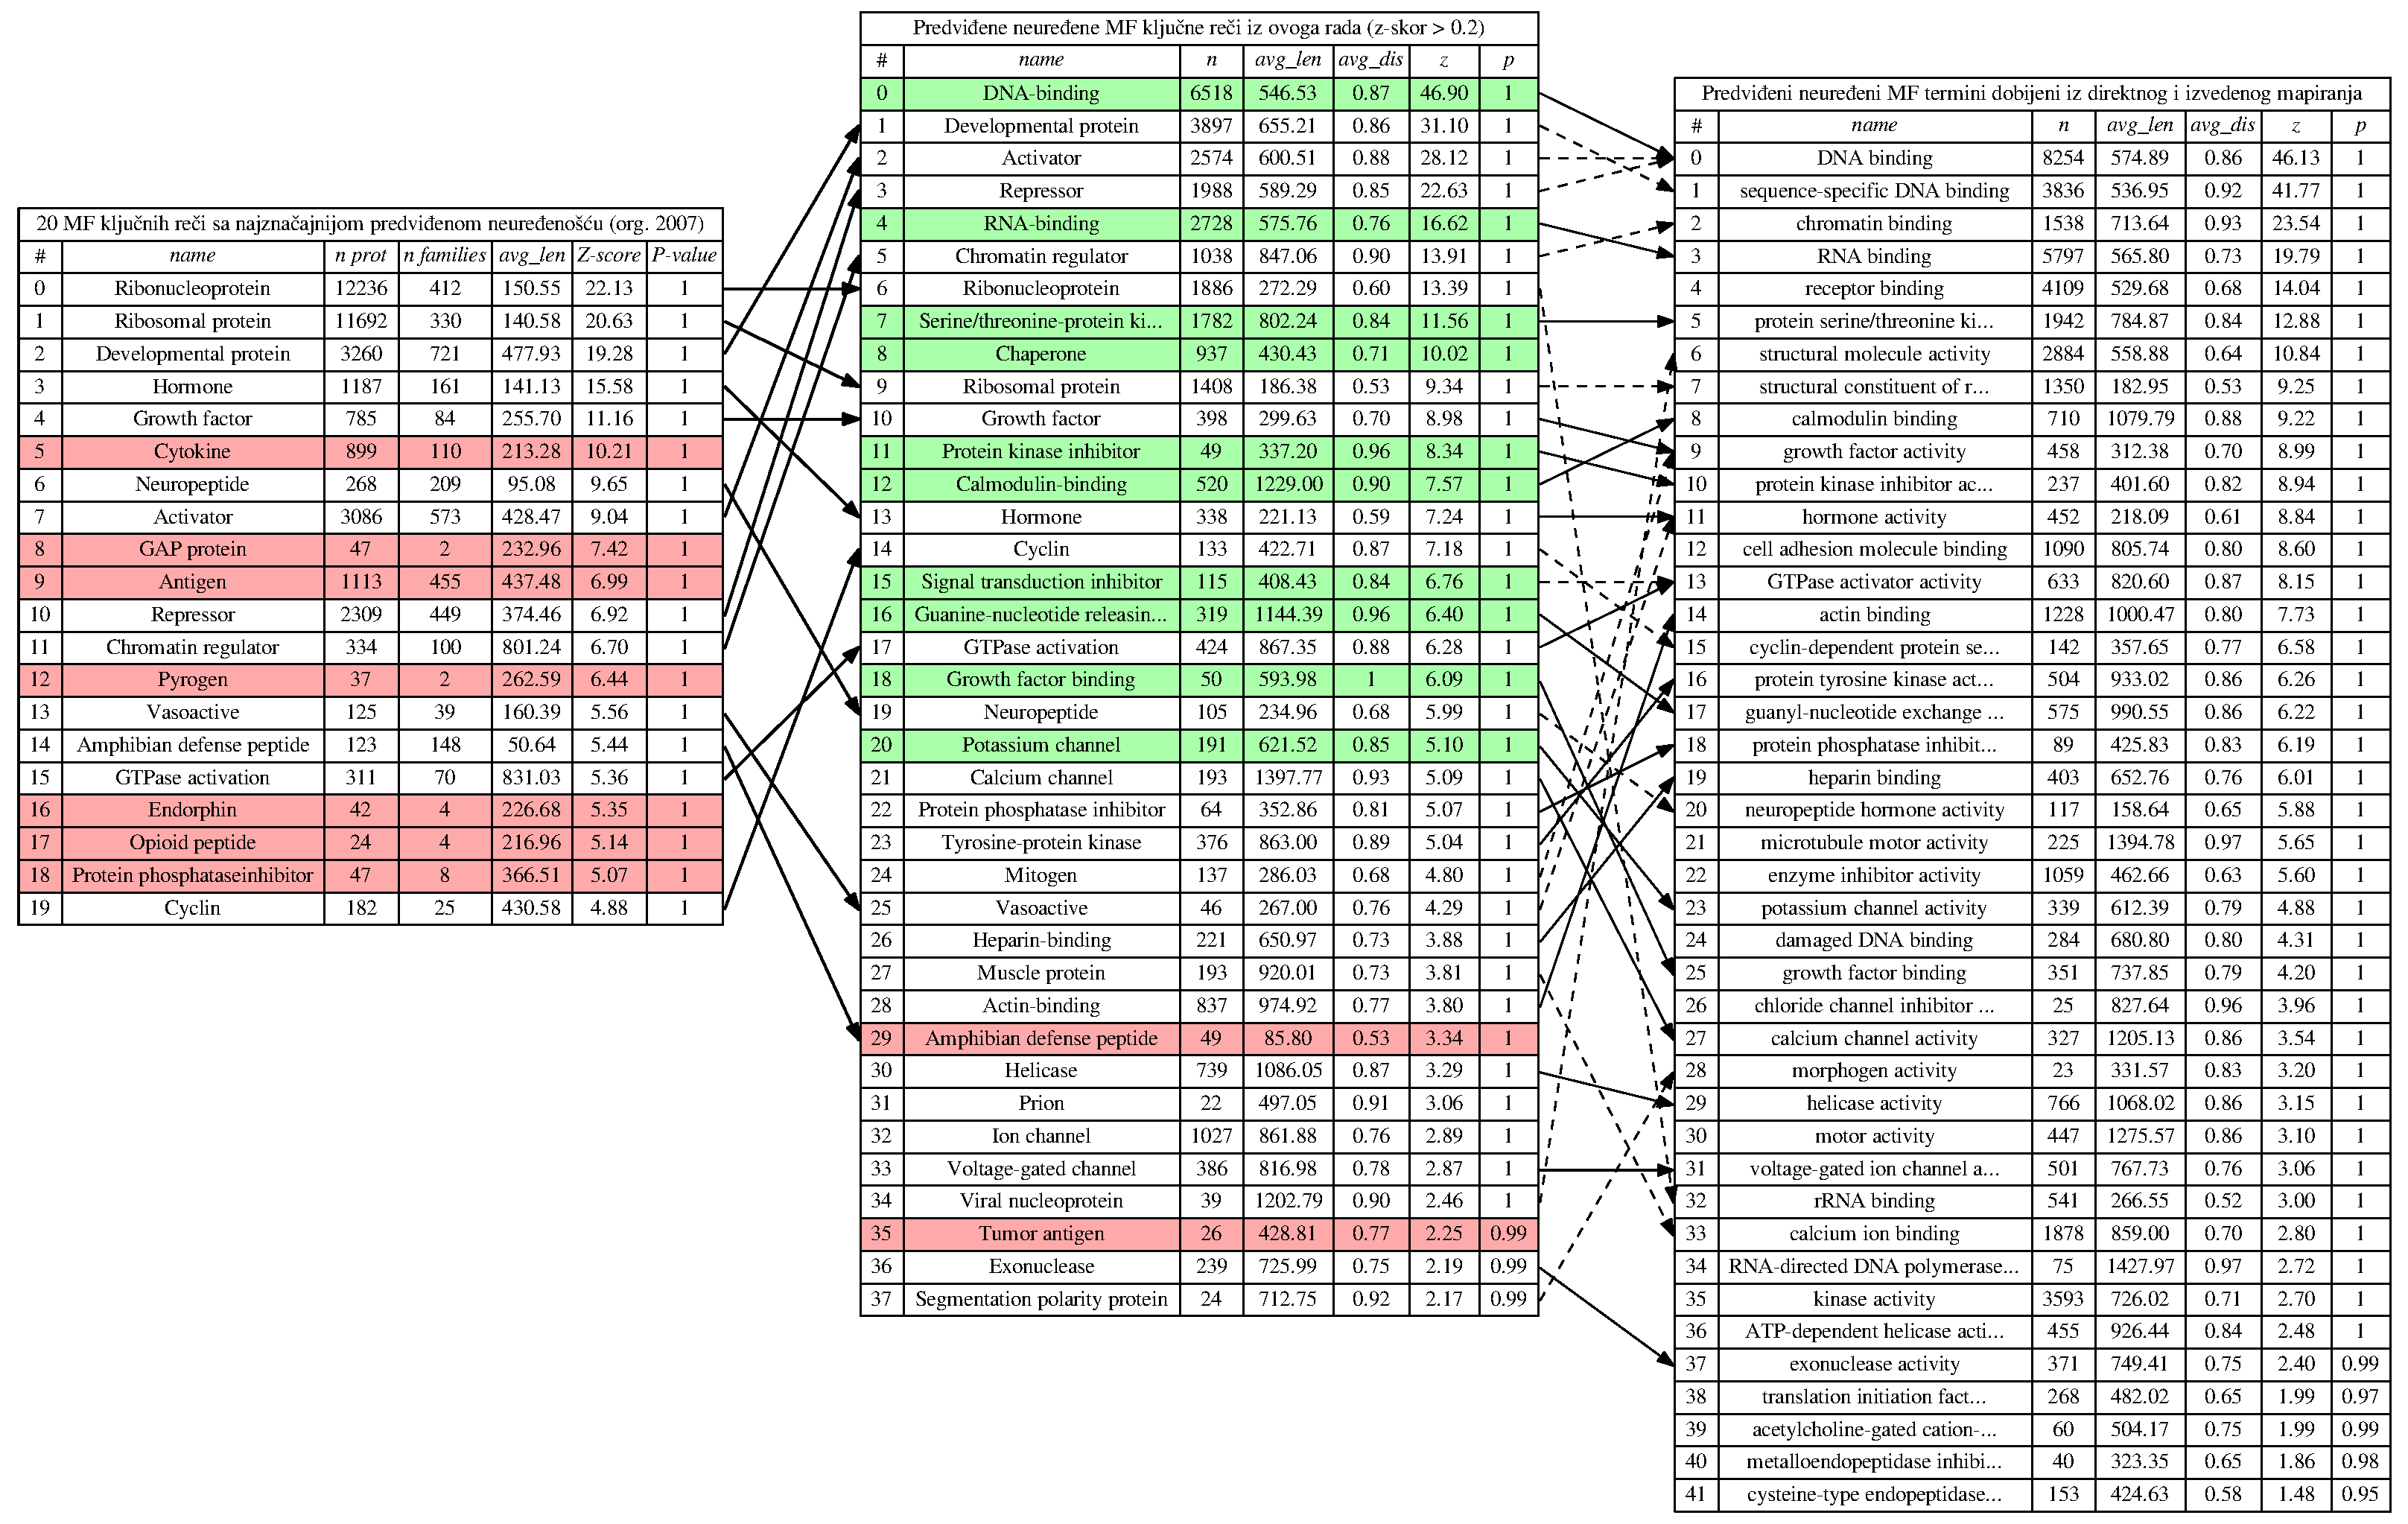
\includegraphics[angle=90, scale=0.45]{Figures/plots/disorder_cmp.pdf}
\decoRule
\caption {
  Poređenje predviđenih neuređenih funkcija
}
\label{fig:disorder_cmp}
\end{figure}

\clearpage

\begin{figure}[th]
\hspace*{-1.0cm} 
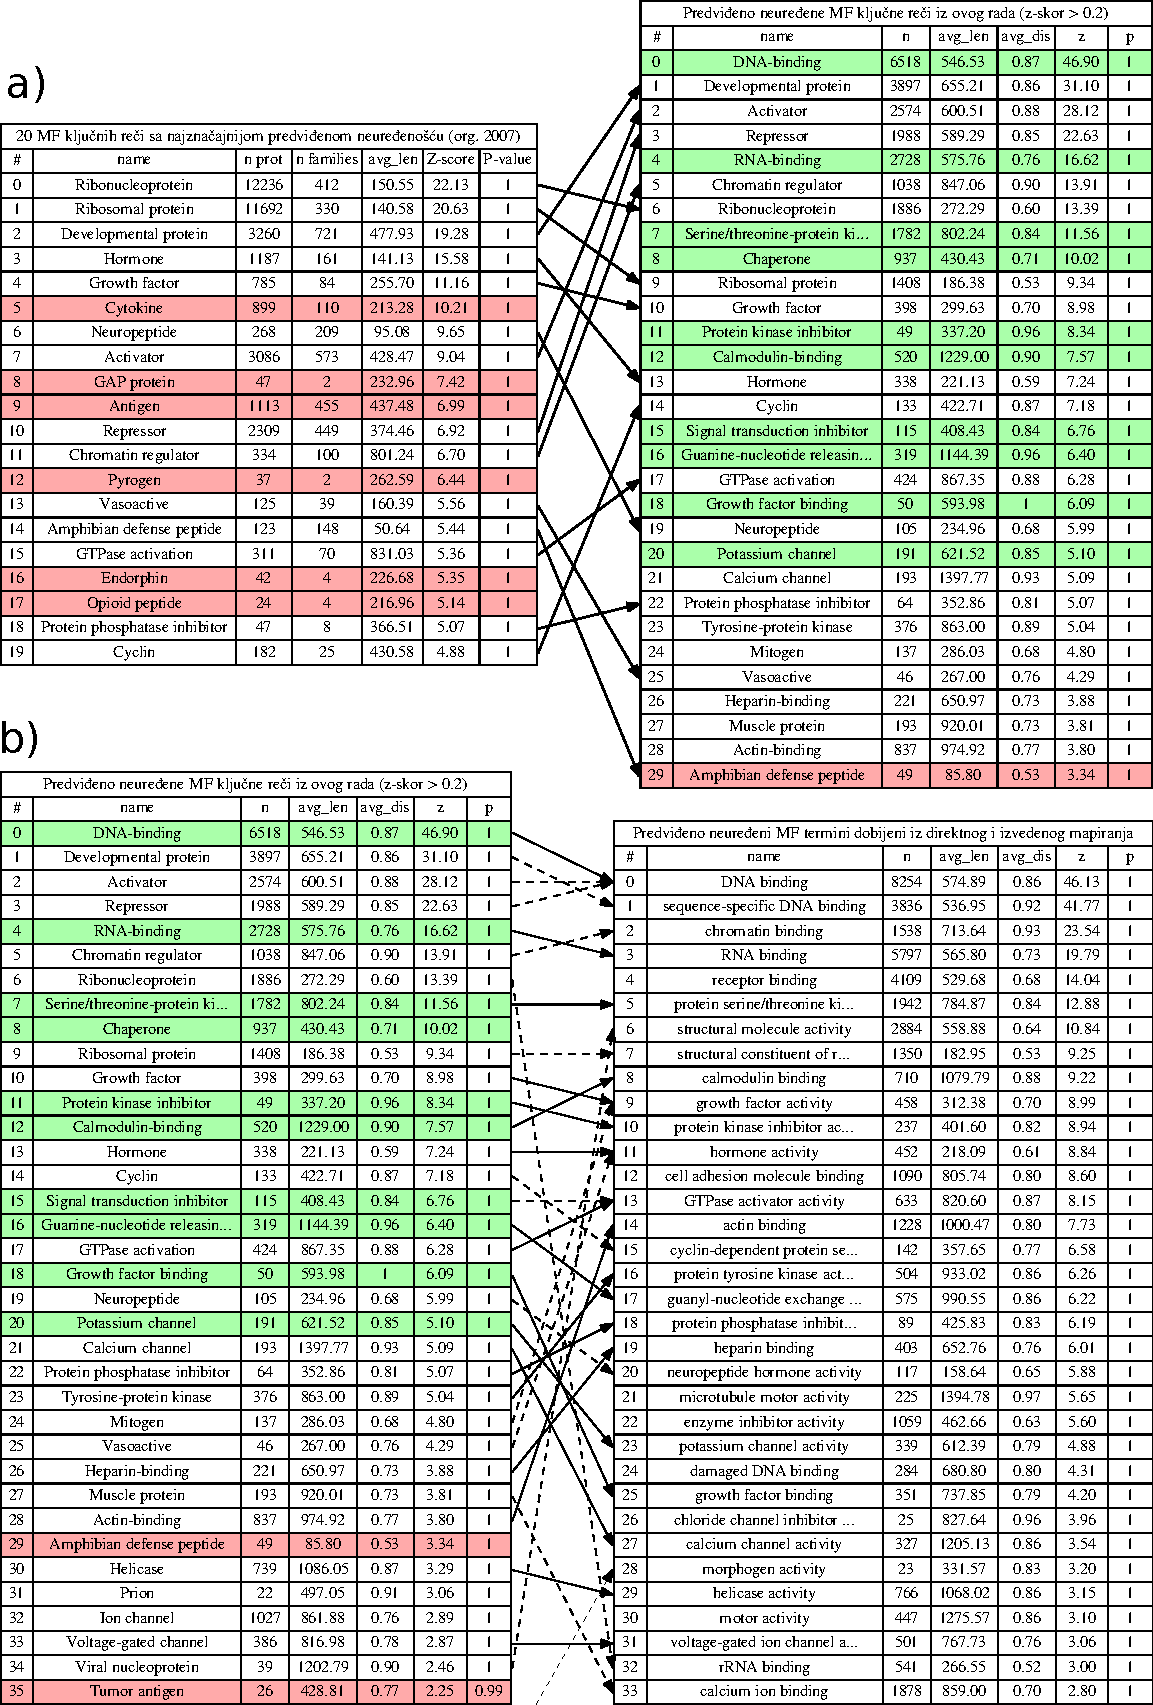
\includegraphics[ scale=0.84]{Figures/plots/disorder_cmp_ab.pdf}
\decoRule
\caption {
  Razdvojeno poređenje predviđenih neuređenih funkcija. Neke tabele su skraćene.
}
\label{fig:disorder_cmp_ab}
\end{figure}

% ------


\begin{figure}[th]
\hspace*{-2.0cm} 
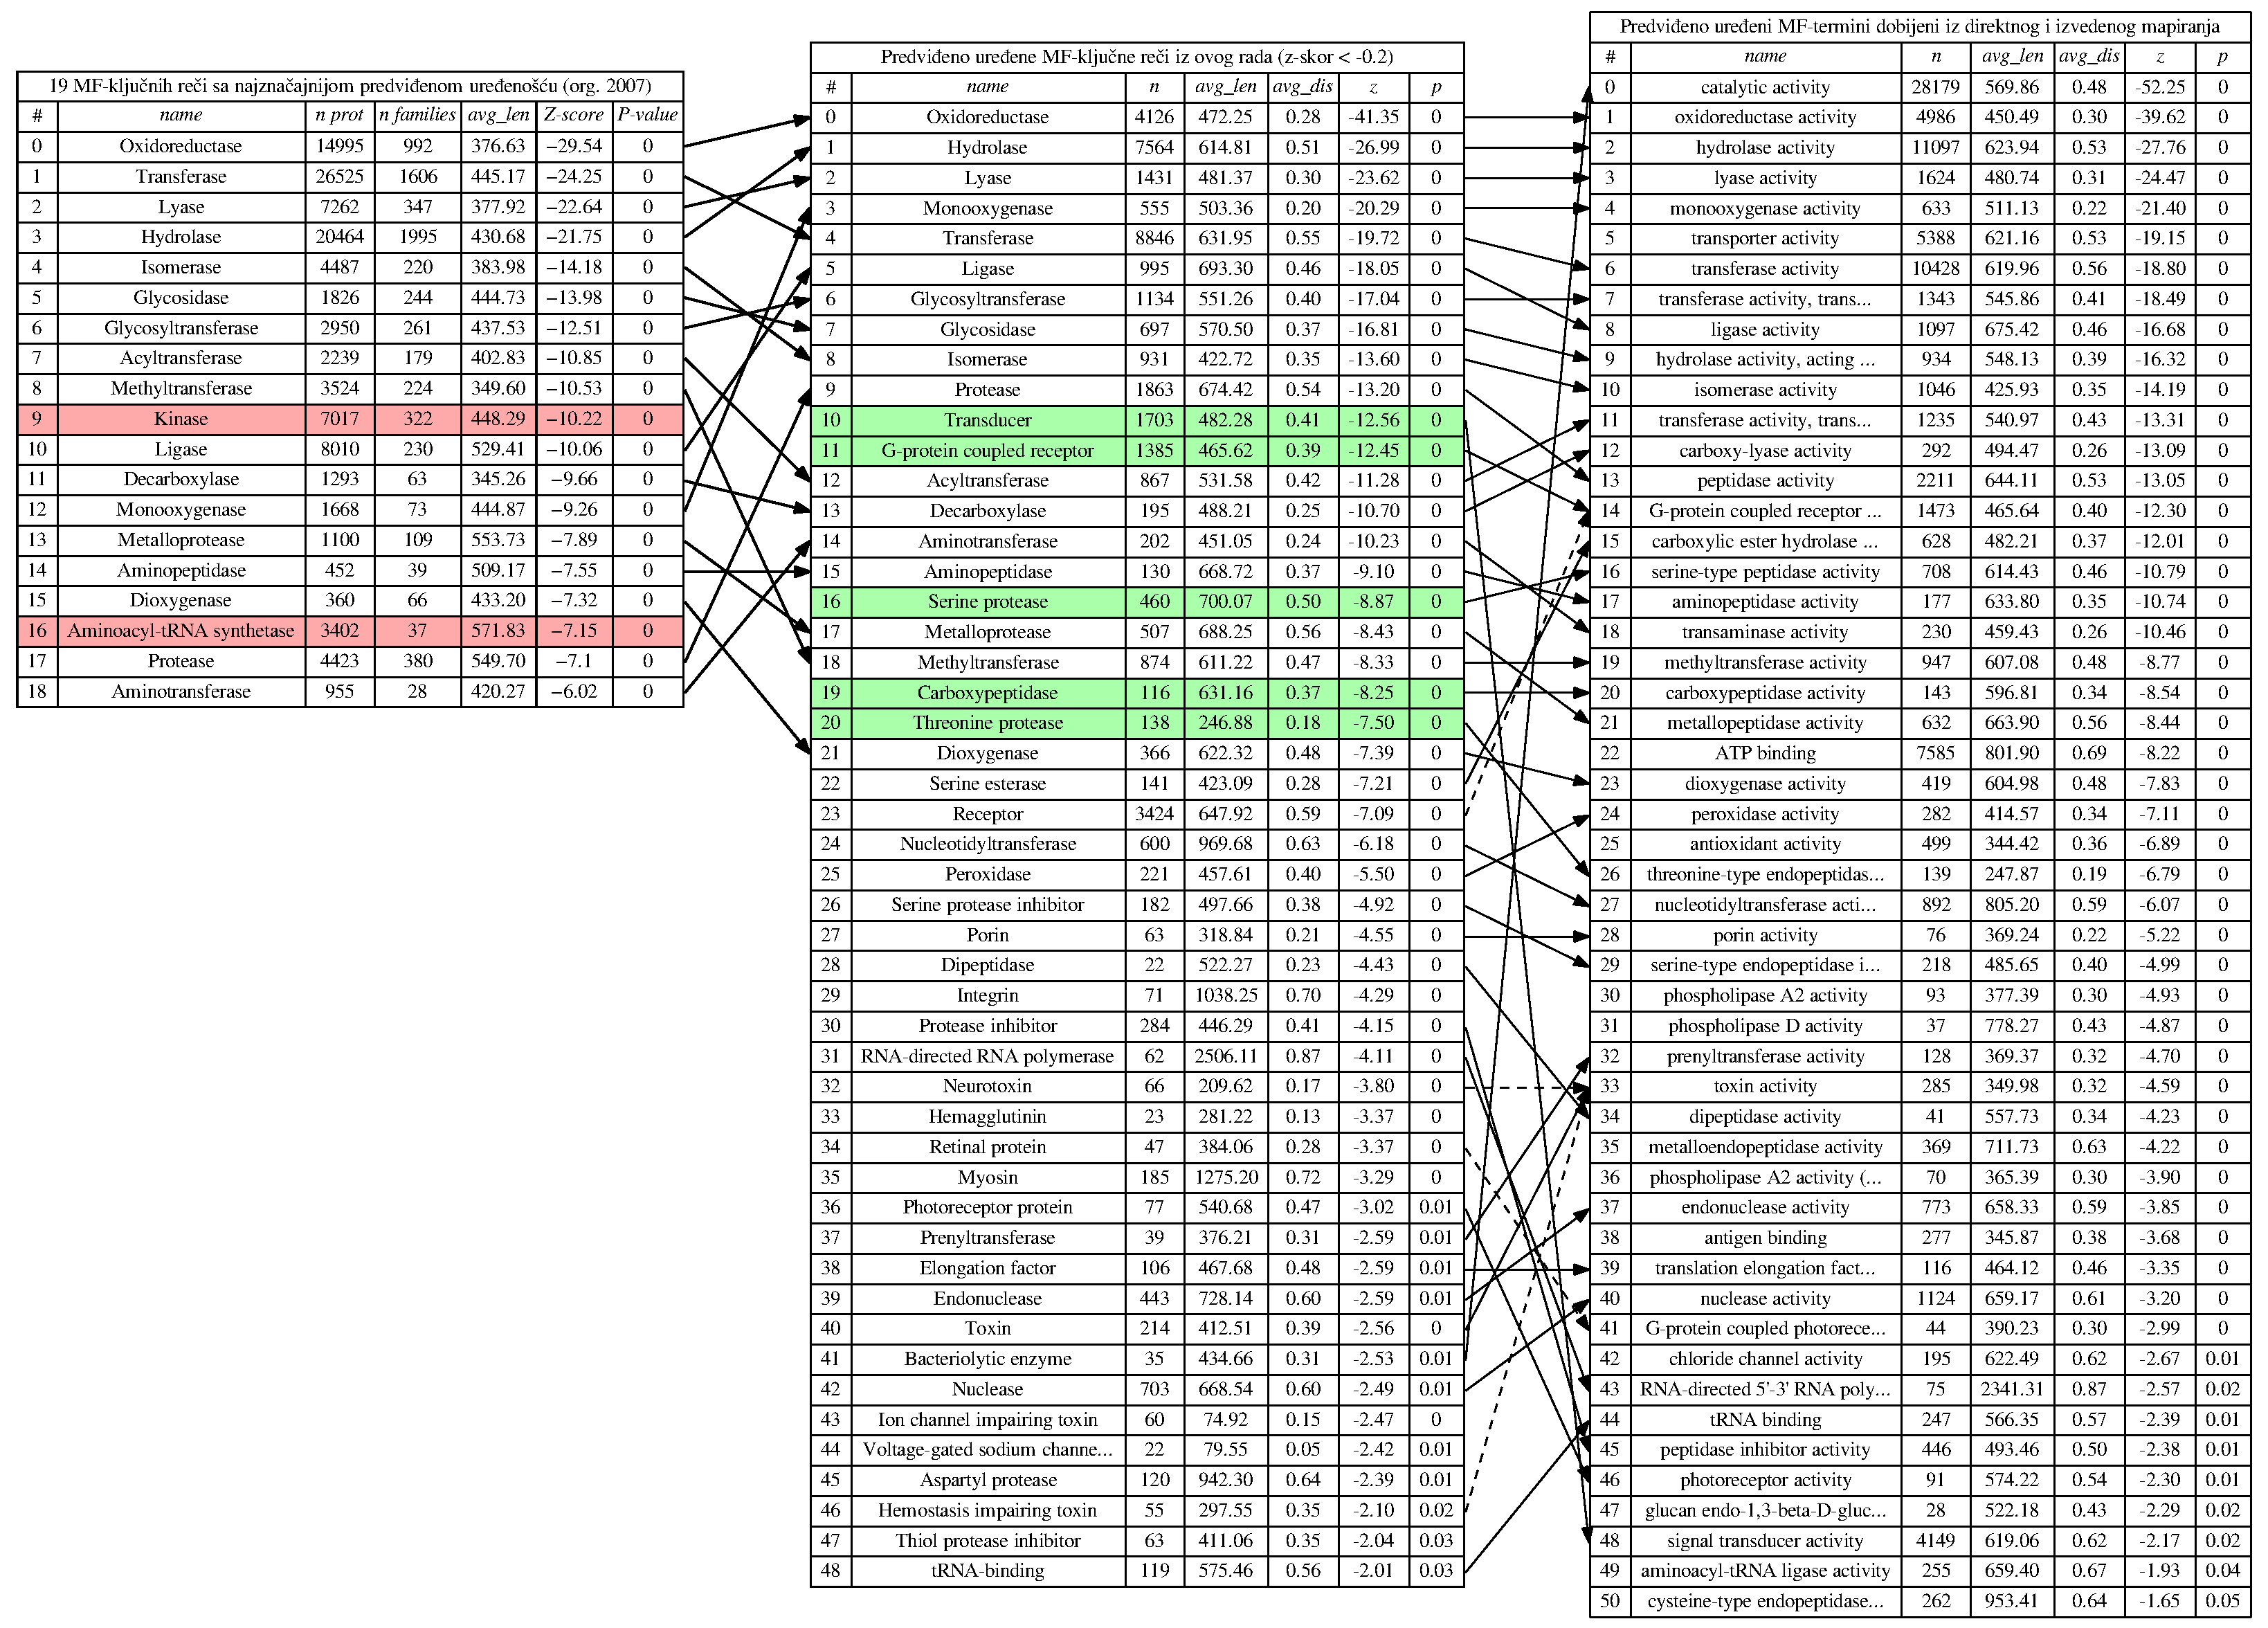
\includegraphics[angle=90, scale=0.45]{Figures/plots/order_cmp.pdf}
\decoRule
\caption {
  Poređenje predviđenih uređenih funkcija
}
\label{fig:order_cmp}
\end{figure}

\begin{figure}[th]
\hspace*{-0.5cm} 
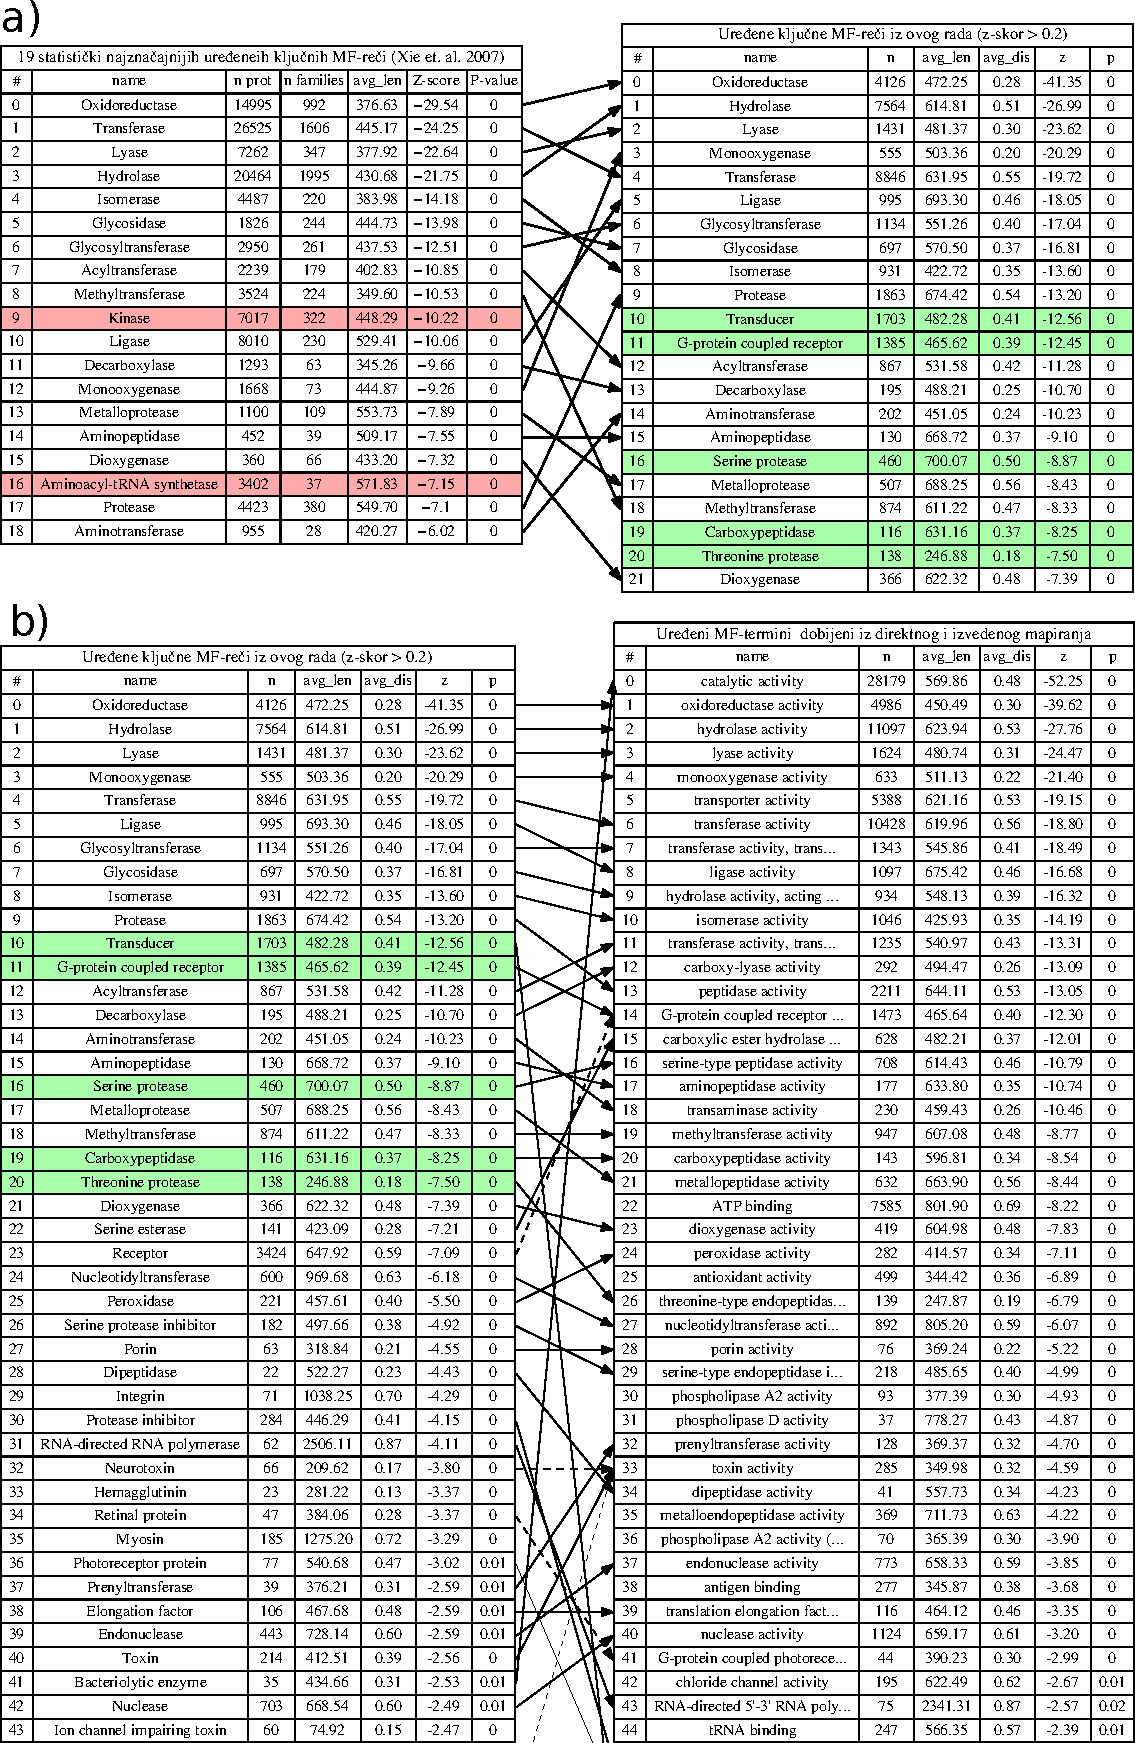
\includegraphics[scale=0.82]{Figures/plots/order_cmp_ab.pdf}
\decoRule
\caption {
  Razdvojeno poređenje predviđenih uređenih funkcija. Neke tabele su skraćene.
}
\label{fig:order_cmp_ab}
\end{figure}


\clearpage

Tabelarni pristup sa Slika \ref{fig:disorder_cmp} i \ref{fig:order_cmp}
prikazuju samo mali podskup svih statistički značajnih MF termina.  Kompletna
analiza grupisanja po MF terminima predstavljena je grafovski, slikama
\file{disorder.svg} i \file{order.svg} koje se nalaze na veb adresi
\cite{rezultati}.  Isečak rezultata \file{disorder.svg} prikazan
je Slikom \ref{fig:disorder_example}.  Pozadinska boja funkcija kodira
\keyword{neuređenost termina}, a kodirana je viridis \cite{viridis} mapiranjem
boja. Viridis mapiranje nulu predstavlja tamno ljubičastom a jedinicu svetlo
žutom pa su tamniji, plavkasti termini  uređeni dok su svetli, zelenkasti
neuređeni.  Rezultujuće \file{.svg} slike su namenjene da budu otvorene u
internet pregledaču.  Držanje kurzora miša iznad funkcija prikazaće dodatne
informacije (ime, definiciju i sinonime), dok će levi klik miša preusmeriti
korisnika na adekvatnu \textit{AmiGO}\footnote{\textit{AmiGO} je skup alat za
pretraživanje i prikazivanje GO termina } ili \uniprot veb stranicu. Desnim
klikom može da se odabere otvaranje stranice u novom tabu pregledača.

\begin{figure}[th]
\hspace*{-2.0cm} 
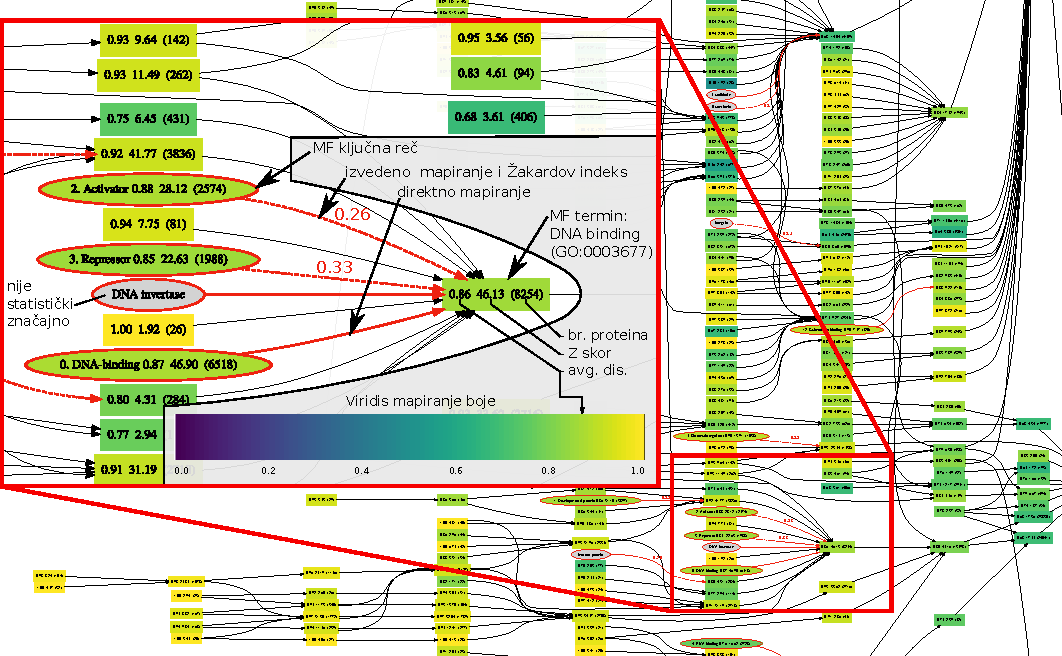
\includegraphics[angle=0, scale=1]{Figures/plots/disorder_example.pdf}
\caption {
  Isečak grafovskog prikaza rezultata (\file{disorder.png}).
}
\label{fig:disorder_example}
\end{figure}


Predloženi $P_L random$ (slučajni) model testirali smo na nivou ključnih reči
izračunavši $z_{rand}$ i  $p_{rand}$ vrednosti za sve MF ključne reči koje
anotiraju bar 20 proteina. Rezultat poređenja z skor vrednosti između $P_L$
modela ($z$-skor) i $P_L random$ modela ($z_{rand}$-skor) prikazan je na Slici
\ref{fig:PLrand}. Prikazane su samo one MF ključne reči koje su statistički
značajne u odnosu na $p$ ili $p_{rand}$ vrednosti dok su crveno obeležene one
ključne reči koje su statistički značajne po jednoj ali ne i drugoj p
vrednosti.


\begin{figure}[th]
\hspace*{-3.0cm} 
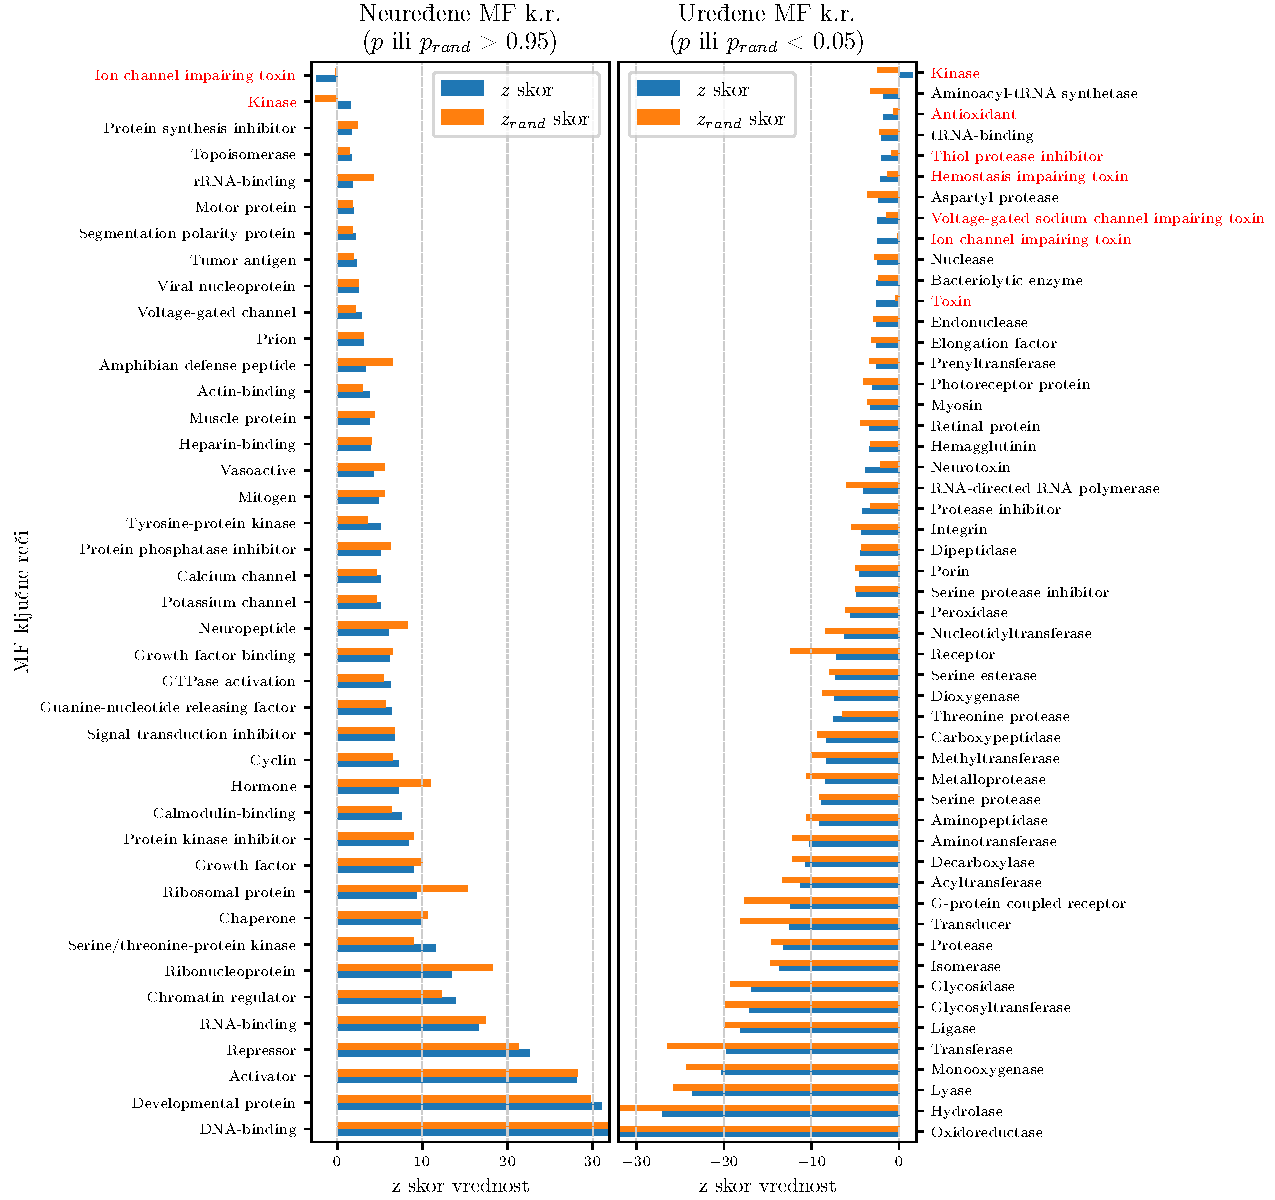
\includegraphics[angle=0, scale=1]{Figures/plots/PL_and_PL_rand.pdf}
\caption {
  Poređenje $PL$ i $PL_{random}$ modela nad statistički značajnim predviđenim (ne)uređenim MF ključnim rečima
}
\label{fig:PLrand}
\end{figure}




\chapter{Diskusija} % Main chapter title

\label{Diskusija} % For referencing 

\section{Međusobno upoređivanje MF ključnih reči}

Razmotrimo prvo Sliku \ref{fig:order_cmp_ab}a koja pokazuje da se originalni
rezultati i novi rezultati ne razlikuju bitno za predviđeno uređene MF ključne
reči. Međutim, razlike koje postoje kao i veći izuzeci (\textit{Kinase} i
\textit{Aminoacyl-tRNA synthetase} )  mogu biti posledica drugačijih podataka,
ali i modifikacije metoda originalne analize ili čak kombinacije oba faktora.
Pronalaženje egzaktnog uzorka ovih razlika zahteva dodatno istraživanje koje
prevazilazi obim ovog rada.

Sa druge strane, predviđeno \keyword{neuređene} MF ključne reči prikazane na
Slici \ref{fig:disorder_cmp_ab}a imaju znatno više razlika u odnosu na
originalne rezultate.  Šest originalnih MF ključnih reči nije identifikovano u
novim rezultatima. Ipak, \textit{Antigen} u novoj verziji ključnih reči ne
postoji dok su četiri ključne reči izbačene iz analize jer anotiraju ispod 10
CAFA3 proteina (minimum je 20).  Preostala, crvena MF ključna reč
\textit{Cytokine} ima p vrednost 0.49 što je veliko odstupanje od originalnih
rezultata. Značajnu razliku predstavljaju zeleno obeležene MF ključne reči koje
se ne javljaju u originalnim rezultatima, a nalaze se među 20 statistički
najznačajnijih novih rezultata. Među njima je preovlađujući motiv \textit{binding}, 
što se ne poklapa sa originalnim rezultatima. Za razliku od GO termina,
ključne reči ne sadrže datum dodavanja ili izmene pa ne možemo da proverimo da
li su u pitanju nove ključne reči koje nisu postojale 2006. godine.


\section{Upoređivanje MF ključnih reči i GO termina}

Rezultati prikazni Slikama \ref{fig:disorder_cmp_ab}b i
\ref{fig:order_cmp_ab}b sugerišu značajno poklapanje za statistički
najznačajnije funkcije. Kao što je očekivano, sličnost rezultata $z$-skor i
neuređenost tj. \textit{avg\_dis} pogotovo su izraženi za funkcije koje anotiraju
slične skupove proteina. Veća nepoklapanja prisutna su prvenstveno kod ključnih
reči čije je mapiranje problematično zbog razlika u nomenklaturi. Na primer,
ključna reč \textit{Bacteriolytic enzyme} nalazi se na 42. mestu dok se njen
direktno mapirani MF termin \textit{catalytic activity} nalazi na prvom mestu.

\section{Grafovski prikaz MF termina}

Grafovski prikaz na slikama \file{disorder.svg} i \file{order.svg} pruža
detaljan uvid u kompleksne hijerarhijske odnose između MF termina. Ovaj prikaz otkriva
strukture koje inače ne bi bile uočene.  Opštije MF funkcije visoke statističke
značajnosti okarakterisane su kompleksnom grafovskom strukturom potomaka. Ipak,
treba naglasiti da ovu strukturu čine isključivo statistički značajni termini
jer bi suprotno rezultat bio  teško saglediv.

\section{Statistička značajnost, neuređenost i broj proteina}

Prosek neuređenih proteina tj. \textit{avg\_dis} (neuređenost) otkriva da
funkcija ne mora da bude pretežno neuređena ili uređena da bi rezultat ($F_J$)
bio statistički značajan.  Na primer, MF termin \textit{hydrolase activity}
(Slika \ref{fig:order_cmp_ab}a) ima $z$-skor $-27.76$, međutim sadrži $53\%$
neuređenih proteina. Ipak, prosečna dužina anotiranih proteina je 624, a
verovatnoća da protein te dužine bude klasifikovan kao neuređen je 0.75.
Takođe, veličina skupa anotiranih proteina (11 097 za \textit{hydrolase
activity}) povećava statističku značajnost rezultata. Verovatno je da veliki
broj proteina smanjuje disperziju što vodi ka većim $z$-skor vrednostima.  Ovo
je posebno izraženo kod MF termina \textit{catalytic activity} na Slici
\ref{fig:order_cmp_ab}a.  Iz ovih razloga smatramo da je neophodno uzeti sve
parametre u obzir, a ne samo $z$-skor ili $p$ vrednost.

\section{$P_Lrandom$ model}

Sličnost rezultat $P_L$ i $P_L random$ modela prikazana je na Slici
\ref{fig:PLrand}. Veća odstupanja \\$z_{rand}$-skora kod ključnih reči
\textit{Ribonucleoprotein, Ribosomal protein, Hormone} i drugih ogledaju se
povećanom statističkom značajnošću. Ovo se može objasniti znatno
nižom prosečnom dužinom skupa anotiranih proteina (manje od 300 AK), dok se na
Slici \ref{fig:PL2} uočava da je $P_L random$ verovatnoća niža za proteine
kraće od 300 AK.  Obrnuto, uređene MF ključne reči globalno imaju niži
$z_{rand}$-skor (veću statističku značajnost) što se takođe može objasniti
kombinacijom globalno veće prosečne dužine proteina i većom $P_L random$
verovatnoćom (Slika \ref{fig:PL2}). 

MF ključna reč \textit{Kinase} predstavlja zanimljivo odstupanje jer $P_L
random$ model predviđa statistički značajnu uređenost iako je prosek neuređenih
proteina 0.71 i $P_L$ model predviđa neuređenost. Takođe, MF termin $Kinase
activity$ je statistički značajno neuređena ($P_L$ model).

\section{Klasifikacija neuređenog proteina}

Definicija \ref{pdis_def} neuređenosti proteina iz Potpoglavlja
\ref{naredno} nije uvek idealna.  Na primer, ako je dužina proteina 35 AK, a
neuređenost je predviđena celom dužinom, onda je jasno da nema potrebe eliminisati
protein iz analize već ga treba svrstati kao neuređeni.  Takođe, ako je protein
dug 50 AK i sadrži predviđeni neuređeni region od 35 AK, onda treba
pretpostaviti da neuređenost igra ulogu u funkciji. Ovi granični slučajevi čine
suviše mali procenat proteina u CAFA3 podksupu pa je opravdano zanemariti ih.
Međutim, procentualno \swissprot sadrži značajno više kratkih proteina što nas
navodi da istaknemo ovaj problem.

\section{Nastavak istraživanja}

Razvoj novih metaprediktora neuređenosti \cite{Meng_c2017} svakako je razlog za
nastavak istraživanja. Testiranje novih metoda analize, korišćenje drugih,
većih skupova podataka i novih metaprediktora može rezultirati interesantnim
rezultatima. Prikaz dobijenih rezultata bi trebalo da uključi razvoj
korisničkog interfejsa koji omogućuje interaktivno istraživanje, poređenje i
povezanost sa drugim resursima. Vizuelna komparacija različitih rezultata u
grafovskom obliku samo je jedan od problema koje treba rešiti.

Računarsko istraživanje veze između funkcije i tipa neuređenosti je naredni
pravac koji treba istražiti. Ipak, prediktori koji predviđaju tip neuređenosti
prema saznanjima autora još ne postoje. Iz tog razloga buduće istraživanje
treba da bude fokusirano na njihov razvoj.




%----------------------------------------------------------------------------------------
%	THESIS CONTENT - APPENDICES
%----------------------------------------------------------------------------------------

\appendix % Cue to tell LaTeX that the following "chapters" are Appendices

% Include the appendices of the thesis as separate files from the Appendices folder
% Uncomment the lines as you write the Appendices

% % Appendix A

\chapter{Frequently Asked Questions} % Main appendix title

\label{AppendixA} % For referencing this appendix elsewhere, use \ref{AppendixA}

\section{How do I change the colors of links?}

The color of links can be changed to your liking using:

{\small\verb!\hypersetup{urlcolor=red}!}, or

{\small\verb!\hypersetup{citecolor=green}!}, or

{\small\verb!\hypersetup{allcolor=blue}!}.

\noindent If you want to completely hide the links, you can use:

{\small\verb!\hypersetup{allcolors=.}!}, or even better: 

{\small\verb!\hypersetup{hidelinks}!}.

\noindent If you want to have obvious links in the PDF but not the printed text, use:

{\small\verb!\hypersetup{colorlinks=false}!}.

%\include{Appendices/AppendixB}
%\include{Appendices/AppendixC}

%----------------------------------------------------------------------------------------
%	BIBLIOGRAPHY
%----------------------------------------------------------------------------------------

\renewcommand{\bibname}{Bibliografija}


\printbibliography[heading=bibintoc]


%----------------------------------------------------------------------------------------

\end{document}  
